\documentclass[11pt]{article}

% ---------------------------------------------------------------------------
% Packages
% ---------------------------------------------------------------------------
\usepackage{fontspec}
\usepackage{microtype}
\usepackage[margin=1in]{geometry}
\usepackage{graphicx}
\usepackage{amsmath,amssymb}
\usepackage{booktabs}
\usepackage{array}
\usepackage{caption}
\usepackage{subcaption}
\usepackage{float}
\usepackage{enumitem}
\usepackage[colorlinks=true, linkcolor=black, citecolor=black, urlcolor=blue]{hyperref}
\usepackage{xurl}
\usepackage[round]{natbib}
\usepackage{setspace}
\usepackage{algorithm}
\usepackage{algpseudocode}

\setlength{\parindent}{0pt}
\setlength{\parskip}{0.6em}

\newcommand{\dbar}{\ensuremath{\bar d}}

\title{\textbf{Deep Neural Network Surrogates for Approximate Bayesian Computation:\\
A Simulation Study for Mutation-Rate Estimation\\
in Markov Branching Processes}}
\author{}
\date{}

\begin{document}

\maketitle

\begin{abstract}
\citet{lu2023} applied GPS-ABC \citep{meeds2014}, a Gaussian-process surrogate
for approximate Bayesian computation (ABC), to estimating mutation rates in a
two-type Markov branching process (MBP). Its central device is a substitution: inside the ABC-MCMC acceptance
step, an expensive MBP simulator is replaced by a Gaussian process (GP)
surrogate fit to a small design of simulator outputs. This paper asks whether a
neural network can perform that same substitution, and, more usefully, when
doing so actually helps. We develop a heteroscedastic multilayer-perceptron
surrogate, calibrated by split-conformal prediction \citep{lei2018}, that takes
the Gaussian process's place inside the same ABC-MCMC sampler with no other
change to the inference procedure, and we evaluate it in two simulation
studies.

The first study reproduces the constant-mutation-rate benchmark of
\citet{lu2023}, replicated with Monte Carlo standard errors reported throughout
\citep{morris2019}. There the neural surrogate's point-estimation mean squared
error is statistically indistinguishable from GPS-ABC's in seven of nine
tested configurations -- nominally lower in five of those seven and higher in
the other two, neither direction resolved beyond simulation noise -- and at
the largest tested mutation rate it is better by a margin that clearly exceeds
that noise (up to $60\%$ lower MSE, a gap of $5.8$--$8.1$ Monte Carlo standard
errors). The neural surrogate nonetheless returns tighter $95\%$ credible
intervals in all nine configurations, and its own regression calibration is
near-exact -- but posterior coverage of those intervals tells a different
story: both surrogates under-cover at the smallest tested culture count and
recover toward nominal as the culture count grows to match their training
data, a genuine limitation we measure directly rather than infer from
regression diagnostics, all at the same two-to-three-order-of-magnitude
speedup over exact ABC-MCMC that the Gaussian process already provides.

The second study turns to the two-stage (piecewise-constant) mutation model, in
which the mutation probability jumps from $p_1$ to $p_2$ at an unknown time
$\tau$ and all three parameters are estimated jointly. Here we report a
deliberately negative result. The neural surrogate fits the response surface to
within $1.05\times$ its irreducible noise floor -- but so do networks spanning
three orders of magnitude in size, and downstream the neural and
Gaussian-process surrogates are statistically tied in seven of nine
parameter-by-truth comparisons at the two-Monte-Carlo-standard-error level,
with the other two favouring the Gaussian process. That verdict survived three
separate corrections to the pipeline -- the mutation-time convention, the
summary statistic, and the activation selected under it -- each of which
measurably improved the surrogate without changing the conclusion. We argue
that this is the expected outcome whenever surrogate error ceases to be the
binding constraint. What binds instead is the model's intrinsic
identifiability: $p_2$ is well determined, while $p_1$ and $\tau$ are recovered
poorly by every method tested. Every method also over-covers its credible
intervals, most severely for the weakly identified $\tau$, a limitation we
diagnose as a property of the ABC acceptance kernel rather than a deficiency of
the surrogate's own predictive calibration, which remains near-exact
throughout. A further controlled comparison across architecture families --
feedforward, convolutional, and recurrent surrogates, motivated by where each
is known to help in the simulation-based-inference literature -- finds that
neither a convolutional nor a recurrent inductive bias improves on the
architecture-agnostic feedforward network for this three-input problem, which
is the outcome the parameters' lack of any real spatial or temporal structure
predicts.

Taken together, the two studies say when a neural surrogate should be preferred
to a Gaussian process inside ABC, and what the coverage gap implies for
deploying conformally calibrated surrogates inside likelihood-free samplers
more generally. Code, data, and a fully scripted reproduction pipeline are
available at \url{https://github.com/sletch1/DNN-ABC-mutation-rates}.
\end{abstract}

\noindent\textbf{Keywords:} approximate Bayesian computation; likelihood-free
inference; surrogate modeling; conformal prediction; heteroscedastic
regression; simulation study; Markov branching process

% =============================================================================
\section{Introduction}
\label{sec:intro}
% =============================================================================

Approximate Bayesian computation (ABC) makes Bayesian inference possible for
stochastic models whose likelihood is intractable but which can be simulated
forward \citep{beaumont2002,marjoram2003,marin2012}. The basic ABC-MCMC sampler
\citep{marjoram2003} accepts a proposed parameter $\theta'$ in proportion to how
closely a simulated summary statistic $S(\theta')$ matches the observed
statistic $S_{\mathrm{obs}}$. That simplicity carries a price: every iteration
costs one or more forward simulations. When the simulator is expensive, this
per-iteration cost dominates the runtime of the entire analysis and can put a
full posterior exploration out of reach altogether.

\citet{lu2023} study this problem for a two-type Markov branching process (MBP)
model of microbial mutation, used to estimate the per-division mutation
probability from Luria--Delbr\"uck-style fluctuation experiments. Their exact
simulator (their Algorithm~2) simulates the branching process cell by cell, and
a single call takes anywhere from a fraction of a second to several minutes
depending on the parameter regime. To make ABC-MCMC tractable, they apply
\textbf{GPS-ABC} \citep{meeds2014}: fit a Gaussian process (GP) regression
surrogate to a modest design of simulator outputs, then substitute the GP's
predictive mean and variance for the simulator inside the MCMC acceptance
step. Every iteration becomes a GP prediction rather than a simulator call,
which is where their reported two-to-three-order-of-magnitude speedup comes
from.

The Gaussian process, however, brings a scaling limitation that is well known
and, for this application, binding: fitting an $n$-point GP costs $O(n^3)$ and
querying it costs $O(n)$ per point, for the na\"ive dense implementation used in
practice at this problem size. Two consequences follow, and the second is the
more damaging. The first is a ceiling on the design; \citet{lu2023} report being
limited to roughly $50$--$200$ points for exactly this reason. The second is
that the ceiling bites hardest where relieving it is most expensive. They note
that GPS-ABC can in fact be \emph{less} accurate than plain ABC-MCMC when the
surrogate's design is built from the expensive exact simulator, precisely
because so few exact-simulator calls can be afforded for that design. A cubic
fitting cost is therefore not merely an inconvenience of implementation; it
propagates into the accuracy of the inference it was introduced to accelerate.
This motivates the question the present paper asks:

\begin{quote}
\emph{Can a neural network surrogate replace the Gaussian process inside this
same ABC-MCMC procedure, and if so, under what conditions does it help?}
\end{quote}

A feedforward network carries neither cost. It has no cubic fitting term, and
its query cost is \emph{flat} in the size of its training set, so it can be
trained on substantially more simulator output than a GP can afford at a matched
computational budget; it also extends naturally to higher-dimensional summary
functions, where a GP's curse of dimensionality is most acute. Neither property
is free, however. A GP's predictive variance is a direct consequence of the
Gaussian-process prior and requires no separate calibration step, whereas a
neural network's predictive uncertainty must be constructed and calibrated
explicitly if it is to play the same role inside the ABC acceptance kernel. That
requirement, rather than the regression itself, is what makes the substitution
non-trivial, and it is what Section~\ref{sec:method} is principally about.

\paragraph{Contributions.} This paper makes five contributions. We build
a heteroscedastic neural-network surrogate, calibrated by split-conformal
prediction \citep{lei2018}, that substitutes for the Gaussian process inside
\citeauthor{lu2023}'s ABC-MCMC sampler with no other change to the inference
algorithm. We run a one-dimensional simulation study reproducing
\citeauthor{lu2023}'s constant-mutation-rate benchmark directly, comparing four
estimators -- method of moments, maximum likelihood, exact ABC-MCMC, and
GPS-ABC -- against the neural surrogate on estimation accuracy,
credible-interval length, coverage, and wall-clock cost. We then run a second
simulation study on the two-stage mutation model that is the original paper's
actual multi-parameter contribution, estimating $(p_1,p_2,\tau)$ jointly, and
we report, honestly and without tuning it away, that the neural surrogate's
advantage does \emph{not} carry over to that regime; we pair that report with
a measurement of the data's irreducible noise floor that explains why. Finally,
rather than assume it, we test whether a convolutional or recurrent
architecture improves on the architecture-agnostic feedforward surrogate in
that same regime, motivated by where such architectures are known
to help elsewhere in the simulation-based-inference literature, and find
that neither does.

\paragraph{Related work.} GPS-ABC \citep{meeds2014} is one instance of a
broader line of work using Gaussian processes to reduce simulator calls in
likelihood-free inference: \citet{wilkinson2014} models the ABC log-likelihood
surface directly rather than the acceptance kernel, \citet{gutmann2016}'s BOLFI
frames the design problem as Bayesian optimization over where to place the next
expensive simulation, and \citet{jarvenpaa2021} extends this to noisy,
parallel-batch likelihood evaluations. All three inherit the same $O(n^3)$
fitting cost this paper's Introduction opens with; none substitutes a neural
surrogate for the GP, which is the specific substitution this paper studies. A
separate and now much larger literature bypasses the GP-versus-network choice
entirely by learning the posterior (or likelihood, or likelihood ratio)
directly with a neural density estimator trained on simulator draws --
\emph{neural} simulation-based inference
\citep{papamakarios2016,greenberg2019,cranmer2020}, implemented in
practice through toolkits such as \texttt{sbi} \citep{tejerocantero2020}. These
methods are \emph{amortized}: training cost is paid once, and posteriors for
new data are then produced without any additional simulation or MCMC, which
GPS-ABC, DNN-ABC and exact ABC-MCMC alike cannot offer, since each requires a
fresh MCMC run per observed data set. Section~\ref{sec:sim1D_results} below adds an amortized neural posterior
estimator, trained on the same simulation budget, to the comparison this
paper otherwise restricts to the surrogate-inside-MCMC design, to make that
trade-off concrete rather than assumed. The comparison is also motivated by a finding from that literature that bears directly on this
paper's own results: \citet{talts2018}'s simulation-based calibration protocol
and \citet{hermans2022}'s large-scale audit of neural SBI methods both report
that posterior approximations -- neural or otherwise -- routinely pass
weaker regression-level diagnostics while failing to cover the true parameter
at the stated rate once checked directly. Section~\ref{sec:sim1D_coverage}'s
distinction between the surrogate's own regression coverage and the ABC
posterior's coverage is an instance of exactly this failure mode, measured
here for a GP/DNN-surrogate-based sampler rather than a neural density
estimator.

The paper proceeds in that order. Section~\ref{sec:background} reviews the MBP
model and GPS-ABC. Section~\ref{sec:method} develops the general neural
surrogate framework. Sections~\ref{sec:sim1D} and \ref{sec:sim3D} report the
constant-rate and two-stage simulation studies. Section~\ref{sec:discussion}
discusses implications and limitations, and Section~\ref{sec:repro} describes
the reproducible pipeline accompanying this paper.

% =============================================================================
\section{Background: ABC for the Markov Branching Process Model}
\label{sec:background}
% =============================================================================

\subsection{The mutation model and the observed statistic}

Following \citet{lu2023}, a population initiated by a single wild-type cell
grows for a fixed observation period under a two-type Markov branching process
(MBP). Three quantities govern it. The first is the per-division mutation
probability $p$, the rate at which a dividing wild-type cell produces a mutant
daughter instead of a wild-type one; it is the estimand throughout this paper.
The second is the division-rate parameter $a$, which sets the overall time scale
of growth. The third is the mutant relative growth rate $\delta$, the ratio of
the mutant lineage's growth rate to the wild type's. We refer the reader to \citet{lu2023} for the full stochastic-process
construction and for their Algorithm~2 (an exact, cell-by-cell simulator,
slow) and Algorithm~4 (a fast approximate simulator using distributional
shortcuts), both of which we re-implement in Python and validate directly
against their original R/MATLAB output (Section~\ref{sec:validation}).

An experiment consists of $J$ independently plated parallel cultures, each
grown from a single wild-type cell for the same fixed time. Culture $j$ yields
a final wild-type count $Z_j$ and mutant count $X_j$. Following
\citeauthor{lu2023}, we work with the single scalar summary statistic
\[
\dbar \;=\; \frac{1}{J}\sum_{j=1}^{J} \sqrt{X_j / Z_j},
\]
which is well behaved across the many orders of magnitude spanned by $p$ and is
the statistic used throughout their ABC procedure. One further transformation is
worth stating explicitly, because every regression in this paper inherits it: we
model $\log_{10}\dbar$ rather than $\dbar$ itself. The reason is that
$\log_{10}\dbar$ varies smoothly and close to linearly in $\theta \equiv
\log_{10} p$ (their Figure~2), and a target that is smooth and nearly linear in
its input is one that both Gaussian-process and neural-network regression fit
considerably better.

\subsection{ABC-MCMC and GPS-ABC}
\label{sec:abcmcmc}

Write $\theta = \log_{10} p$ for the (log-scale) parameter of interest. Given
an observed statistic $\dbar_{\mathrm{obs}}$, classical ABC-MCMC
\citep{marjoram2003} targets the approximate posterior
\[
\pi_\epsilon(\theta \mid \dbar_{\mathrm{obs}}) \;\propto\; \pi(\theta)\,
\mathbb{E}_{S \sim F_\theta}\!\left[K_\epsilon\!\left(\dbar_{\mathrm{obs}}, S\right)\right],
\]
by drawing a single summary $S$ from the simulator at each proposed $\theta$
and weighting it with a smoothing kernel $K_\epsilon$ of bandwidth $\epsilon$
that down-weights simulated statistics far from $\dbar_{\mathrm{obs}}$. The
"exact" baseline used throughout this paper is not this literal kernel
average: it is Wood's \citep{wood2010} \emph{synthetic likelihood}. At each
proposed $\theta'$, we draw $n_s$ pilot simulations from $F_{\theta'}$, take
their sample mean $m(\theta')$ and variance $v(\theta')$, and score
$\dbar_{\mathrm{obs}}$ against a matched Gaussian,
\[
\hat\pi_\epsilon(\dbar_{\mathrm{obs}} \mid \theta') \;=\;
\mathcal{N}\!\left(\dbar_{\mathrm{obs}};\; m(\theta'),\; \epsilon^2 + v(\theta')\right).
\]
This is a deliberate choice, not an approximation of convenience: it is
exactly the likelihood form Section~\ref{sec:method}'s surrogates use, with a
predicted variance $\sigma_\phi(\theta')^2$ in place of the pilot-simulation
variance $v(\theta')$, so that every column of
Tables~\ref{tab:mse1D}--\ref{tab:cov1D} shares one likelihood and differs only
in how $(m(\theta), v(\theta))$ is obtained. Algorithm~\ref{alg:abcmcmc}
states the shared Metropolis--Hastings sampler (following
\citeauthor{lu2023}): a truncated-exponential prior on $\theta$ and a
truncated-normal random-walk proposal, wrapped around this likelihood.

\begin{algorithm}[H]
\caption{ABC-MCMC for $\theta=\log_{10}p$ (Metropolis--Hastings, synthetic likelihood)}
\label{alg:abcmcmc}
\begin{algorithmic}[1]
\State Initialize $\theta_0$; set tolerance $\epsilon$, simulator-repeat count $n_s$.
\For{$t = 1, \dots, T$}
  \State Propose $\theta' \sim q(\cdot \mid \theta_{t-1})$ (truncated-normal random walk)
  \State Obtain $(m(\theta'), v(\theta'))$: either (a) simulate $n_s$ times from $F_{\theta'}$ and take their sample mean and variance (synthetic likelihood; \citealp{wood2010}), or (b) evaluate a surrogate's predicted mean and variance $(\mu_\phi(\theta'), \sigma_\phi(\theta')^2)$ (Section~\ref{sec:method})
  \State Compute acceptance probability
  \[
  \alpha \;=\; \min\!\left(1,\; \frac{\pi(\theta')\,q(\theta_{t-1}\mid\theta')}{\pi(\theta_{t-1})\,q(\theta'\mid\theta_{t-1})}\,\cdot\,\frac{\hat\pi_\epsilon(\dbar_{\mathrm{obs}} \mid \theta')}{\hat\pi_\epsilon(\dbar_{\mathrm{obs}} \mid \theta_{t-1})}\right)
  \]
  \State Set $\theta_t = \theta'$ with probability $\alpha$, else $\theta_t = \theta_{t-1}$
\EndFor
\State \Return posterior sample $\{\theta_t\}_{t=B+1}^{T}$ after discarding $B$ burn-in draws
\end{algorithmic}
\end{algorithm}

Under this shared likelihood, step 4(a) draws $n_s$ fresh simulations from the
true process at $\theta'$ to estimate $(m,v)$ -- the expensive step.
\textbf{GPS-ABC} \citep{meeds2014}, applied by \citet{lu2023} to the
branching-process model studied here, instead fits a Gaussian process to a
design $\{(\theta_i, \dbar_i)\}_{i=1}^n$ of simulator outputs \emph{once},
before sampling begins, and at every iteration uses step 4(b): the GP's
posterior predictive mean $\mu_{\mathrm{GP}}(\theta')$ and variance
$\sigma_{\mathrm{GP}}(\theta')^2$ take the place of $(m(\theta'), v(\theta'))$
directly, no pilot simulation required. This is the mechanism by which the
GP's predictive variance enters the acceptance probability directly, and it
sets the standard that any replacement surrogate must meet. What is required
is not merely an accurate mean but a well-calibrated variance, because the two
failure modes are asymmetric and both corrupt the posterior: an overconfident
$\sigma$ inflates the acceptance rate at parameter values the surrogate does
not actually know well, while an underconfident one over-rejects. A surrogate
that predicts the response perfectly and its own uncertainty badly is not a
usable substitute here.

The GP's fitting cost is $O(n^3)$ in the design size $n$ and its per-query
cost during MCMC sampling is $O(n)$, both because the predictive mean and
variance require solving a linear system involving the full training kernel
matrix. \citet{lu2023} report design sizes of roughly 50 points in the
one-dimensional constant-rate case and up to about 200 points (via a
Latin-hypercube design) in a four-parameter piecewise-rate extension, and note
that GPS-ABC trained on the exact simulator can be \emph{less} accurate than
uncorrected ABC-MCMC in some one-dimensional configurations -- plausibly a
consequence of the small design the cubic cost permits when the design points
themselves come from the expensive exact simulator.

% =============================================================================
\section{A Neural-Network Surrogate for ABC}
\label{sec:method}
% =============================================================================

We replace the Gaussian process in step 4(b) of Algorithm~\ref{alg:abcmcmc}
with a neural network $f_\phi$ trained to predict both the mean and the variance
of $\log_{10}\dbar$ as a function of the parameter(s) of interest. The
substitution is deliberately minimal: the sampler, the acceptance ratio, and the
convolution with $\epsilon^2$ are all exactly those of GPS-ABC, so that any
difference in the results that follow is attributable to the surrogate and to
nothing else. We refer to the resulting procedure as \textbf{DNN-ABC}. The two
subsections below supply the two things the network needs in order to stand in
for the GP: an input-dependent predictive variance, and a guarantee that the
variance is calibrated.

\subsection{Heteroscedastic regression}
\label{sec:hetero}

$f_\phi$ has two output heads, $\mu_\phi(x)$ and $\log\sigma^2_\phi(x)$, where
$x$ is $\theta=\log_{10}p$ alone (Section~\ref{sec:sim1D}) or the parameter
vector $(\log_{10}p_1, \log_{10}p_2, \tau)$ (Section~\ref{sec:sim3D}); in
both studies the surrogate is a direct function of the parameters being
inferred, with no derived features. Both heads are trained
jointly by minimizing the Gaussian negative log-likelihood
\begin{equation}
\label{eq:nll}
\mathcal{L}(\phi) \;=\; \frac{1}{n}\sum_{i=1}^n \left[
\frac{\left(y_i - \mu_\phi(x_i)\right)^2}{2\,\sigma_\phi^2(x_i)}
\;+\; \frac{1}{2}\log \sigma_\phi^2(x_i)
\right],
\end{equation}
where $y_i = \log_{10}\dbar_i$. The difference from a single-output network
trained under squared-error loss is the point of the construction. Equation~\ref{eq:nll}
targets an \emph{input-dependent} predictive variance directly -- the network's
analogue of the GP's posterior variance -- and Section~\ref{sec:sim1D} shows
that this is not a refinement but a requirement: the true
replicate-to-replicate noise in $\log_{10}\dbar$ is far from homoscedastic
across the parameter range, and a Gaussian process carrying a single noise term
cannot represent that shape at all.

\subsection{Split-conformal calibration}
\label{sec:conformal}

Training a variance head is not the same as calibrating one. The head produced
by Equation~\ref{eq:nll} is an approximation to the true conditional variance
learned from a finite training set, and nothing in that objective guarantees it
is well calibrated in finite samples. Since Section~\ref{sec:abcmcmc} established
that the acceptance step consumes this quantity directly, an uncalibrated head is
a defect the sampler will inherit. We therefore apply split-conformal calibration
\citep{lei2018} to correct it. After training on a training split, we form
calibration scores on a held-out calibration split of size $m$,
\[
s_i \;=\; \frac{\left|y_i - \mu_\phi(x_i)\right|}{\sigma_\phi(x_i)}, \qquad i=1,\dots,m,
\]
and set the calibration factor $\hat c$ to the $\left\lceil (m+1)(1-\alpha)
\right\rceil / m$ empirical quantile of $\{s_i\}$, the finite-sample
correction of \citet{lei2018}. The calibrated $(1-\alpha)$ predictive interval
for a new input $x$ is then $\mu_\phi(x) \pm \hat c\, \sigma_\phi(x)$. Provided
the calibration and test points are exchangeable, this construction guarantees
marginal coverage of at least $1-\alpha$ in finite samples, without any
distributional assumption on $f_\phi$'s errors \citep{lei2018}. We use
$\alpha = 0.05$ throughout, and refer to this coverage guarantee as the
surrogate's \emph{regression calibration}, to distinguish it explicitly
from the empirical coverage of the downstream ABC posterior's credible
intervals, a materially different quantity with no equivalent theoretical
guarantee (Sections~\ref{sec:sim1D_calib} and \ref{sec:sim3D_coverage}
report both, and the distinction between them is central to the honest
limitation reported in Section~\ref{sec:sim3D_coverage}).

The calibrated $\hat c\,\sigma_\phi(x)$ is used as the surrogate's predictive
standard deviation both when reporting regression calibration and when
plugging $\sigma_\phi(\theta')$ into the ABC-MCMC acceptance kernel of
Algorithm~\ref{alg:abcmcmc}, so that the same calibrated uncertainty that is
validated in Sections~\ref{sec:sim1D_calib} and \ref{sec:sim3D} is what
actually enters the sampler.

\subsection{Ground-truth data and simulator validation}
\label{sec:validation}

In both studies, ground truth is generated by the exact/slow MBP simulator
(\citeauthor{lu2023}'s Algorithm~2), re-implemented in Python from the original
R/MATLAB code. A ported simulator is an assumption until it is checked, and
every number in this paper rests on it, so the port is validated in two ways
before any surrogate is trained: the closed-form plating-time equation is solved and compared
against the R implementation's solver output (agreement to $3\times10^{-5}$),
and the simulator's simulated $\dbar$ means are compared against the
committed ground-truth CSV at matched grid points (Sections~\ref{sec:sim1D}
and \ref{sec:sim3D} report the resulting agreement for each study).

\subsection{Simulation design and reporting}
\label{sec:ademp}

We report both simulation studies following the structure recommended by
\citet{morris2019}: \emph{aims} -- compare five estimators (MOM, MLE, exact
ABC-MCMC, GPS-ABC, DNN-ABC) in Study I, and the two surrogate methods
(GPS-ABC, DNN-ABC) in Study II, where the constant-rate MOM and MLE
estimators do not apply, on point accuracy, interval precision and coverage,
and computational cost, under known ground truth; \emph{data-generating
mechanisms} -- the validated MBP simulator of Section~\ref{sec:validation}, at
the parameter grids specified in Sections~\ref{sec:sim1D_results} and
\ref{sec:sim3D_abc}; \emph{estimands} -- the mutation probability $p$ (via
$\theta=\log_{10}p$) in Study I, and the two-stage parameters
$(p_1,p_2,\tau)$ jointly in Study II;
\emph{methods} -- the estimators of Section~\ref{sec:abcmcmc} and
\ref{sec:method}, all evaluated on identical simulated data sets within a
cell; and \emph{performance measures} -- MSE and normalized RMSE of $\hat p$,
mean 95\% credible-interval length, empirical coverage, and wall-clock time
per 100 MCMC iterations.

Each cell of each study is evaluated over $R$ independent replicated data
sets ($R=40$ in Study I, $R=16$ per truth triple in Study II), and, following
\citeauthor{morris2019}'s recommendation, we accompany every MSE comparison
with its Monte Carlo standard error (MCSE), computed as the usual standard
error of a sample mean applied to the per-replicate squared errors: writing
$e_r = (\hat p_r - p)^2$ for replicate $r=1,\dots,R$ under a given method and
cell, $\widehat{\mathrm{MSE}} = R^{-1}\sum_r e_r$ has
$\widehat{\mathrm{MCSE}} = \mathrm{sd}(e_r)/\sqrt{R}$. For the head-to-head
comparison between the two surrogates in each cell, we report the gap
$\widehat{\mathrm{MSE}}_{\mathrm{GPS}} - \widehat{\mathrm{MSE}}_{\mathrm{DNN}}$
in units of its own combined Monte Carlo standard error $\sqrt{\mathrm{MCSE}_{\mathrm{GPS}}^2
+ \mathrm{MCSE}_{\mathrm{DNN}}^2}$ (a $\Delta/\mathrm{SE}$ column in
Table~\ref{tab:mse1D}, and Section~\ref{sec:sim3D_abc} for Study II); this is a descriptive diagnostic
of whether a point comparison is resolved at this replicate count, not a
formal hypothesis test, and we use it throughout to avoid over-interpreting
small numerical differences as the replicate count varies across cells and
between the two studies ($R=40$ versus $R=16$).

% =============================================================================
\section{Simulation Study I: One-Dimensional Constant Mutation Rate}
\label{sec:sim1D}
% =============================================================================

The first study reproduces \citeauthor{lu2023}'s original benchmark exactly:
$a=\delta=Z_0=1$ held fixed, and only $p$ varying. Ground truth is
$101$ log-spaced values of $p$ with $\log_{10}p \in [-8,-2]$, ten replicates
each ($1{,}010$ rows total), $J=100$. We split \emph{by replicate} rather than by grid point, which is what keeps the
comparison honest: every value of $p$ then appears in every split, so a split
tests generalisation to fresh noise rather than to an unseen region of the
parameter axis, and no grid point can leak from training into evaluation.
Replicates 1--5 are used for training ($505$ rows), 6--8 for conformal
calibration and early stopping ($303$ rows), and 9--10 are held out for
test-only evaluation ($202$ rows). The GPS-ABC baseline is fit on the identical
replicates 1--8, so that both surrogates see the same data budget; neither ever
sees the test replicates.

\subsection{Architecture, and the one choice that mattered}
\label{sec:arch1D}

The network is a shallow funnel multilayer perceptron: input
$\theta=\log_{10}p$, two GELU-activated dense layers, and the two linear
output heads of Section~\ref{sec:hetero}. Its final width, $32$ then $16$
($626$ parameters), is the outcome of a two-stage search reported across this
section: an activation/normalisation sweep run at a $128$--$64$ baseline
(immediately below), then a capacity sweep of that baseline itself once the
activation question was settled (Section~\ref{sec:arch1D}, ``Is the two-layer
$128$--$64$ network actually needed?''). We report the search in that
order -- activation first, then capacity -- because that is the order it was
run in, and each stage's conclusion held fixed the choice the previous stage
made. The first stage was a controlled search (Table~\ref{tab:arch1D}) against
the mean-curve fit achieved by the GP baseline, holding fixed the goal of
matching or beating the GP's fit to the denoised response curve
$\mathbb{E}[\log_{10}\dbar \mid \theta]$, at the $128$--$64$ width then in use:

\begin{table}[H]
\centering
\caption{Architecture search, one-dimensional model: mean-curve fit MSE
against the denoised response curve (irreducible replicate-noise floor
$\approx 4.7\times 10^{-3}$).}
\label{tab:arch1D}
\resizebox{\textwidth}{!}{%
\begin{tabular}{lrr}
\toprule
Model & Mean-curve MSE & vs.\ GP \\
\midrule
Gaussian process (GPS-ABC baseline) & $3.836\times10^{-4}$ & --- \\
\textbf{DNN, GELU (128, 64), no BatchNorm [selects activation]} & $\mathbf{3.888\times10^{-4}}$ & $+1\%$ \\
DNN ensemble $\times 5$, SiLU (128, 128, 64) & $3.960\times10^{-4}$ & $+3\%$ \\
DNN ensemble $\times 5$, tanh (256, 128) & $4.178\times10^{-4}$ & $+9\%$ \\
DNN, SiLU (128, 128, 64) & $4.400\times10^{-4}$ & $+15\%$ \\
DNN, tanh (64, 64, 32) & $4.435\times10^{-4}$ & $+16\%$ \\
DNN, tanh (256, 128) & $4.503\times10^{-4}$ & $+17\%$ \\
DNN, ReLU + BatchNorm + dropout (64, 64, 32) & $4.352\times10^{-3}$ & $+1035\%$ \\
\bottomrule
\end{tabular}}
\end{table}

The row that determines every downstream comparison in this study is the last
one: an otherwise-reasonable network carrying BatchNorm \citep{ioffe2015} and
dropout fits \emph{eleven times worse} than the same network without them. The
mechanism is specific to this problem rather than general. BatchNorm normalises
per-minibatch statistics, which is useful in deep classification networks; but
on a smooth scalar regression over a one-sided domain -- the $\theta$-grid has a
hard edge at $-8$ -- it injects batch-dependent noise and biases predictions
near that boundary. What closes the gap to the GP is therefore not any choice of
activation function. It is the removal of a component that most practitioners
would have included by default. A follow-up ablation isolating only the activation function
(same 128-64 architecture, no BatchNorm, averaged over three random seeds)
found ReLU, SiLU \citep{elfwing2018}, GELU \citep{hendrycks2016}, and tanh
within $7\%$ of one another ($3.95$--$4.23 \times 10^{-4}$): a statistical tie,
with ReLU marginally ahead. Because accuracy does not separate them, the choice
is made on structural grounds instead. We use GELU for its smoothness, which
matters should the sampler later be adapted to a gradient-based scheme, and for
its immunity to the dead-neuron failure mode, at no measurable accuracy cost in
this setting. ReLU would serve equally well, and we claim nothing from the
ranking. A second architecture-search
round using $7$-network deep ensembles (mean-curve MSE $3.94$--$4.25\times
10^{-4}$ across four ensemble configurations) did not improve on the single
chosen network, so the simpler model is retained throughout.

The network is trained with an Adam optimizer under early stopping on
calibration-split negative log-likelihood, weight decay $10^{-5}$, no
dropout (early stopping and weight decay already control overfitting on this
smooth curve; dropout's injected noise measurably hurt the fit in
preliminary runs).

\paragraph{Why convolutional and recurrent architectures are not tested here.}
Study II (Section~\ref{sec:sim3D_arch}) reports a controlled comparison of
feedforward, convolutional, and recurrent surrogates on the three-input
two-stage problem. We do not repeat that comparison here because it would be
vacuous: with a single scalar input $\theta=\log_{10}p$, a 1-D convolution has
no neighbouring position to convolve over and a recurrent cell has no second
time step to recur into, so both architectures collapse mathematically to the
already-tested single-layer linear map. Building them would relabel, not
extend, the architecture search in Table~\ref{tab:arch1D}.

\paragraph{Is the two-layer 128--64 network actually needed?} Table~\ref{tab:arch1D}
fixes width at $128$--$64$ while sweeping activation and normalisation; width
and depth were never themselves swept. We test that directly in two stages,
holding GELU and no BatchNorm fixed throughout
(\texttt{network/architecture\_search/benchmark\_capacity.py} for the curve-fit
sweep, \texttt{benchmark\_capacity\_confirm.py} for the downstream stage below).
First, a curve-fit sweep from the $128$--$64$ baseline down to a linear control,
averaged over three seeds, against the denoised response curve. Second, a
screen-then-confirm downstream check mirroring the discipline of
Section~\ref{sec:sim3D_act}'s activation search: every candidate is first
screened at this project's own quick-check settings (2 replicates, one
$(p,J)$ cell), and every candidate survives that screen within a factor of
two of the best, so all six are then confirmed at the paper's own
Table~\ref{tab:mse1D} scale -- $40$ replicates, the full $p\times J$ grid,
$600$ MCMC iterations -- with Monte Carlo standard errors attached exactly as
in Section~\ref{sec:ademp}. The exact-simulator baseline is not re-run for
every candidate, since its cost cannot depend on the surrogate's size.

\begin{table}[H]
\centering
\caption{One-dimensional model: does capacity matter? Curve MSE is
against the denoised response curve, mean $\pm$ sd over three seeds. Downstream
MSE and 95\% CI length are DNN-ABC at the same scale as Table~\ref{tab:mse1D}
($40$ replicates/cell, full $p\times J$ grid), one seed per row.}
\label{tab:capacity1D}
\begin{tabular}{lrrrr}
\toprule
Hidden layers & Parameters & Curve MSE ($\times$ GP) & Downstream MSE & Downstream 95\% CI \\
\midrule
GP (GPS-ABC baseline) & --- & $3.836\times10^{-4}$ (---) & $2.702\times10^{-6}$ & $2.137\times10^{-3}$ \\
\textbf{32--16 (deployed)} & \textbf{626} & $\mathbf{3.896\times10^{-4}}$ ($\mathbf{+1.6\%}$) & $\mathbf{1.433\times10^{-6}}$ & $\mathbf{1.300\times10^{-3}}$ \\
128--64 (original) & $8{,}642$ & $4.129\times10^{-4}$ ($+7.6\%$) & $1.514\times10^{-6}$ & $1.308\times10^{-3}$ \\
64--32 & $2{,}274$ & $3.957\times10^{-4}$ ($+3.2\%$) & $1.565\times10^{-6}$ & $1.377\times10^{-3}$ \\
16 (1 layer) & $66$ & $4.460\times10^{-4}$ ($+16.3\%$) & $1.579\times10^{-6}$ & $1.375\times10^{-3}$ \\
8 (1 layer) & $34$ & $4.983\times10^{-4}$ ($+29.9\%$) & $1.668\times10^{-6}$ & $1.393\times10^{-3}$ \\
16--8 & $186$ & $4.508\times10^{-4}$ ($+17.5\%$) & $1.810\times10^{-6}$ & $1.528\times10^{-3}$ \\
Linear (control) & $4$ & $4.672\times10^{-4}$ ($+21.8\%$) & --- & --- \\
\bottomrule
\end{tabular}
\end{table}

Two things follow, and they point in the same direction here. On raw curve fit,
capacity is not merely unnecessary above a small threshold -- it is mildly
\emph{counter-productive} at the original size: $128$--$64$ has the largest gap
to the GP of any two-layer candidate tested ($+7.6\%$), while $32$--$16$, at
$14\times$ fewer parameters, comes closest to matching it ($+1.6\%$). With only
$606$ training rows and a response curve this smooth, the larger network has
more room to overfit, not less. On the downstream task the surrogate is
actually used for, $32$--$16$ is also the best point estimate on both accuracy
and interval length of every candidate tested, $128$--$64$ included -- and
attaching Monte Carlo standard errors to the gap, as Section~\ref{sec:ademp}
does throughout, shows that while this specific edge over $128$--$64$ is not
itself resolved (all nine $\Delta/\mathrm{SE}$ values fall below $0.6$ in
magnitude, nowhere near the $\sim 2$ threshold this paper treats as resolved
elsewhere), nothing in the data argues against it either: $32$--$16$ never
does measurably worse than $128$--$64$ in any cell, on either the curve-fit or
the downstream comparison. Even the nominally worst two-layer candidate,
$16$--$8$ at $46\times$ fewer parameters, is measurably worse than $128$--$64$
in only one of nine cells (the largest-$p$, largest-$J$ cell, where signal is
strongest) and tied in the other eight. Every candidate beats the GP baseline
by a wide, decisive margin on both columns in every cell. Only the linear
control shows a clear, unambiguous cost on curve fit, confirming a
nonlinearity is required somewhere, just not much capacity beyond that.

\textbf{We redeploy on the strength of this table.} $32$--$16$ is the best
point estimate everywhere it can be compared to $128$--$64$ and strictly
better on curve fit, at $14\times$ fewer parameters; no analysis in this paper
can show a cost to making the change, and Occam's razor settles a comparison
this evenly matched in favour of the smaller model. The deployed network is
$32$--$16$; Tables~\ref{tab:mse1D}--\ref{tab:time1D} and every figure in this
study are reported for it, retrained from the same data splits and
re-evaluated at the same paper scale (40 replicates, the full $p\times J$
grid, including the exact-simulator baseline). The $128$--$64$ row above is
retained permanently as the architecture the activation and BatchNorm search
of Table~\ref{tab:arch1D} was actually run against, not as the deployed
model. The honest limit on the redeployment decision itself is the one
already stated: the specific margin by which $32$--$16$ led in this section's
own comparison is not distinguishable from Monte Carlo noise at that
replicate count, so what was established there is that the smaller network is
not worse, not that it is provably better -- a conclusion the paper-scale
retraining above does not overturn: Table~\ref{tab:mse1D} shows the same
pattern of near-ties with two cells of clearly resolved advantage that the
$128$--$64$ network showed, at $14\times$ fewer parameters.

\subsection{Regression calibration}
\label{sec:sim1D_calib}

Table~\ref{tab:fit1D} reports the surrogate's fit and split-conformal coverage
on each data split.

\begin{table}[H]
\centering
\caption{One-dimensional surrogate: fit and 95\% regression coverage by split.}
\label{tab:fit1D}
\begin{tabular}{lrrrr}
\toprule
Split & $n$ & MSE($\log_{10}\dbar$) & MAE($\log_{10}\dbar$) & 95\% coverage \\
\midrule
Train & 505 & 0.00424 & 0.0515 & 0.964 \\
Calibration & 303 & 0.00533 & 0.0538 & 0.954 \\
\textbf{Test} & \textbf{202} & \textbf{0.00434} & \textbf{0.0525} & \textbf{0.9554} \\
\bottomrule
\end{tabular}
\end{table}

The held-out test-set coverage of $0.9554$ ($193$ of $202$ points) is within
sampling noise of the nominal $0.95$, consistent with the finite-sample
guarantee of \citet{lei2018}. Figure~\ref{fig:calib1D} shows the calibrated
$95\%$ band against the test data and the resulting test-set parity, and
compares the surrogate's input-dependent predictive standard deviation to the
GP's flat, homoscedastic one.

\begin{figure}[H]
\centering
\begin{subfigure}{0.48\textwidth}
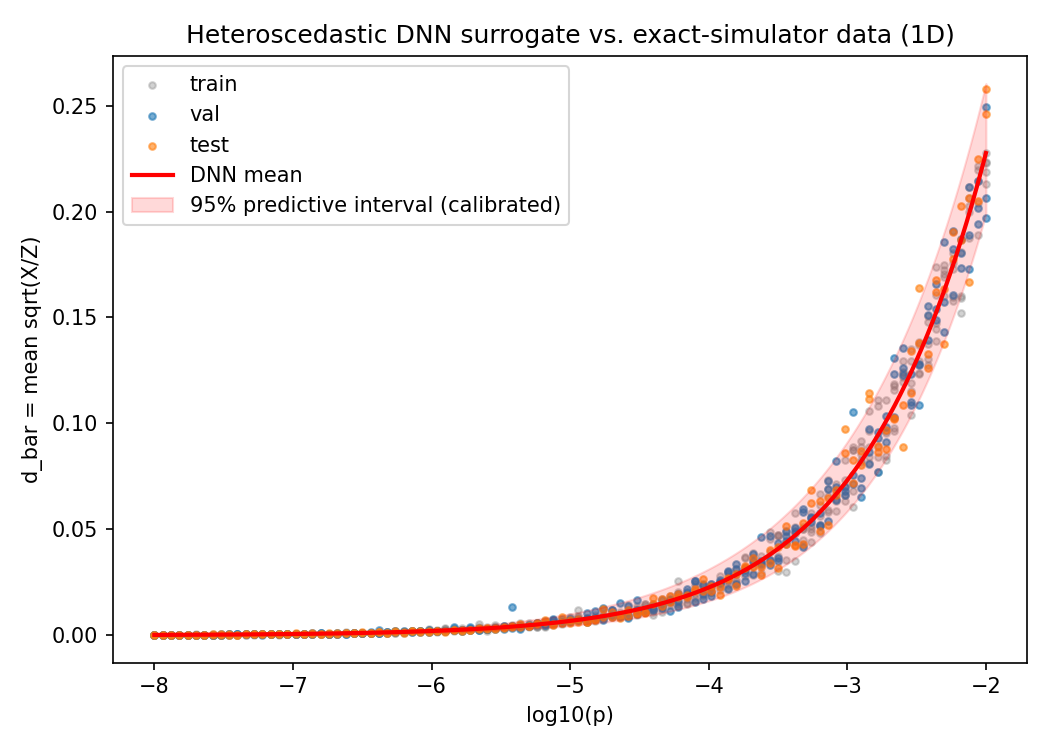
\includegraphics[width=\linewidth]{Models/1D/results/figures/surrogate_fit.png}
\caption{Calibrated 95\% predictive band}
\end{subfigure}\hfill
\begin{subfigure}{0.48\textwidth}
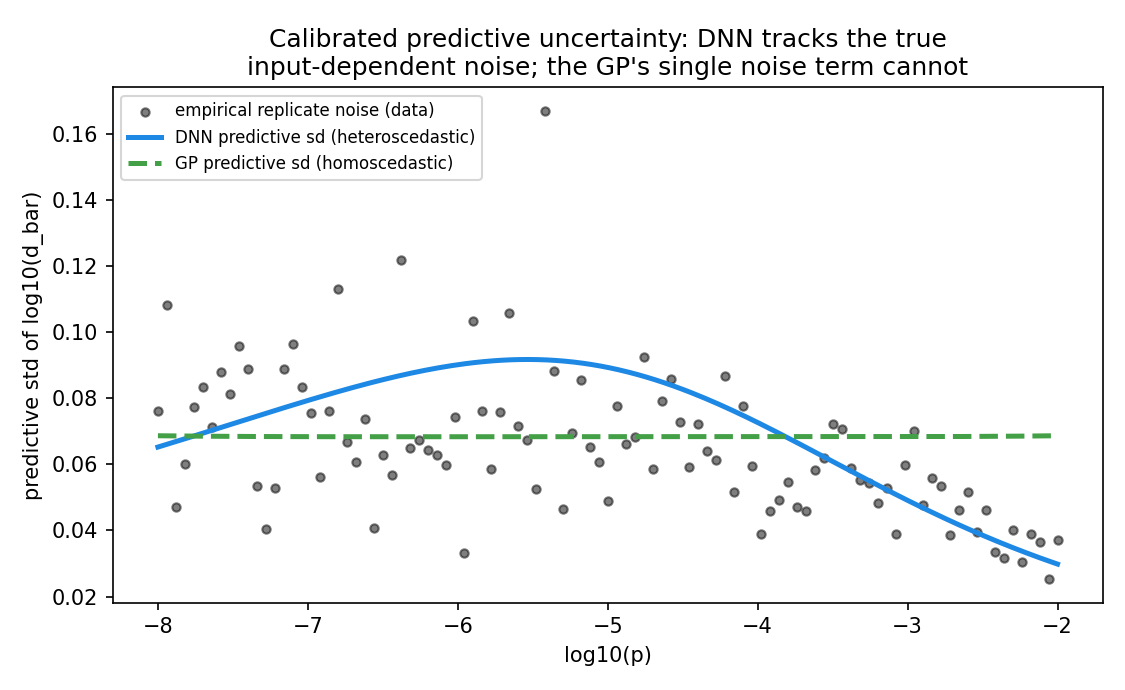
\includegraphics[width=\linewidth]{Models/1D/results/figures/fig_uncertainty.png}
\caption{Input-dependent uncertainty vs.\ the GP}
\end{subfigure}
\caption{One-dimensional surrogate calibration. Left: the calibrated 95\%
predictive band tracks the response curve across the full range of $\theta$.
Right: the network's heteroscedastic predictive standard deviation (which
enters the ABC acceptance kernel directly) tracks the true input-dependent
replicate noise, while the GP's single homoscedastic noise term is flat by
construction.}
\label{fig:calib1D}
\end{figure}

\subsection{ABC simulation results}
\label{sec:sim1D_results}

We ran the full ABC-MCMC / GPS-ABC / DNN-ABC comparison at $40$ independent
replicated data sets per cell, $600$ MCMC iterations ($250$ burn-in), $n_s=6$
simulator repeats per exact-ABC iteration, prior $\theta \sim
\mathrm{TruncExp}$ on $[-5,-2]$ (bounded so that the exact simulator inside
the ABC-MCMC loop remains computationally feasible; both surrogates are
trained on the wider $[-8,-2]$ range and only queried in-range), on the grid
$p \in \{10^{-4}, 10^{-3}, 10^{-2}\} \times J \in \{10, 50, 100\}$. Method of
moments (MOM) and maximum likelihood (MLE) estimators follow \citeauthor{lu2023}'s
closed-form expressions and serve as classical, non-ABC baselines.

\begin{table}[H]
\centering
\caption{Study I, Table 1: MSE of $\hat p$ across five estimators; normalized
RMSE $\sqrt{\mathrm{MSE}}/p$ in parentheses. Bold marks the lower of GPS-ABC
and DNN-ABC in each row. $\Delta/\mathrm{SE}$ is the GPS-ABC$-$DNN-ABC MSE gap
in units of its combined Monte Carlo standard error (Section~\ref{sec:ademp});
values below $\sim 2$ in magnitude are not clearly resolved at $R=40$
replicates.}
\label{tab:mse1D}
\resizebox{\textwidth}{!}{%
\begin{tabular}{rrrrrrrr}
\toprule
$p$ & $J$ & MOM & MLE & ABC-MCMC & GPS-ABC & DNN-ABC & $\Delta/\mathrm{SE}$ \\
\midrule
$10^{-4}$ & 10  & 9.36e-9 (0.97)  & 1.02e-8 (1.01)  & 2.90e-9 (0.54) & 7.02e-9 (0.84) & \textbf{6.61e-9 (0.81)} & 0.07 \\
$10^{-4}$ & 50  & 8.68e-9 (0.93)  & 9.59e-9 (0.98)  & 1.91e-9 (0.44) & 1.88e-9 (0.43) & \textbf{1.78e-9 (0.42)} & 0.23 \\
$10^{-4}$ & 100 & 4.18e-9 (0.65)  & 4.64e-9 (0.68)  & 7.75e-10 (0.28) & 8.21e-10 (0.29) & \textbf{7.83e-10 (0.28)} & 0.14 \\
$10^{-3}$ & 10  & 1.38e-6 (1.17)  & 1.60e-6 (1.26)  & 4.60e-7 (0.68) & \textbf{5.10e-7 (0.71)} & 5.30e-7 (0.73) & $-$0.11 \\
$10^{-3}$ & 50  & 3.21e-7 (0.57)  & 3.85e-7 (0.62)  & 1.15e-7 (0.34) & 1.23e-7 (0.35) & \textbf{1.19e-7 (0.34)} & 0.08 \\
$10^{-3}$ & 100 & 2.71e-7 (0.52)  & 3.29e-7 (0.57)  & 4.33e-8 (0.21) & \textbf{4.29e-8 (0.21)} & 4.35e-8 (0.21) & $-$0.04 \\
$10^{-2}$ & 10  & 3.42e-5 (0.58)  & 4.40e-5 (0.66)  & 2.64e-5 (0.51) & 1.14e-5 (0.34) & \textbf{8.57e-6 (0.29)} & 0.86 \\
$10^{-2}$ & 50  & 7.71e-6 (0.28)  & 1.17e-5 (0.34)  & 4.78e-6 (0.22) & 5.98e-6 (0.24) & \textbf{2.36e-6 (0.15)} & \textbf{5.80} \\
$10^{-2}$ & 100 & 4.01e-6 (0.20)  & 6.08e-6 (0.25)  & 2.62e-6 (0.16) & 6.22e-6 (0.25) & \textbf{2.48e-6 (0.16)} & \textbf{8.12} \\
\bottomrule
\end{tabular}}
\end{table}

Two readings of this table must be kept apart, and conflating them is the error
the $\Delta/\mathrm{SE}$ column exists to prevent. DNN-ABC's point estimate is
numerically lower than GPS-ABC's in seven of the nine cells and marginally
higher in the other two ($p=10^{-3}$ at $J=10$ and $J=100$) -- but nominally
lower is not the same as reliably better, and in both directions the
$\Delta/\mathrm{SE}$ column shows the comparison is clearly resolved beyond
simulation noise in only two cells: $p=10^{-2}$ at $J=50$ and $J=100$, where
the gap favours DNN-ABC by $5.8$ and $8.1$ combined Monte Carlo standard
errors. In the other seven cells, including the two nominal reversals,
$|\Delta/\mathrm{SE}| < 0.9$, so none of those differences -- in either
direction -- is distinguishable from noise at $R=40$ replicates: a near-exact
statistical tie, consistent with a GP fit on $\sim 800$ points already being
close to optimal at these smaller mutation rates. The one regime where the
surrogates are reliably distinguished is the largest tested rate, $p=10^{-2}$,
where DNN-ABC's nRMSE is $0.15$--$0.16$ against GPS-ABC's $0.24$--$0.25$. Both
surrogates match, and in several cells slightly improve on, the exact
ABC-MCMC baseline, and all ABC-based methods substantially outperform the
classical MOM/MLE estimators -- reproducing \citeauthor{lu2023}'s central
finding that ABC dominates the classical estimators for this model.

\begin{table}[H]
\centering
\caption{Study I, Table 2: mean length of the 95\% ABC credible interval for
$\hat p$. Bold marks the shorter of GPS-ABC and DNN-ABC.}
\label{tab:ci1D}
\begin{tabular}{rrrrr}
\toprule
$p$ & $J$ & ABC-MCMC & GPS-ABC & DNN-ABC \\
\midrule
$10^{-4}$ & 10  & 2.39e-4 & 1.14e-4 & \textbf{1.01e-4} \\
$10^{-4}$ & 50  & 1.56e-4 & 1.11e-4 & \textbf{1.04e-4} \\
$10^{-4}$ & 100 & 1.21e-4 & 1.23e-4 & \textbf{1.14e-4} \\
$10^{-3}$ & 10  & 2.51e-3 & 1.32e-3 & \textbf{9.39e-4} \\
$10^{-3}$ & 50  & 1.53e-3 & 1.32e-3 & \textbf{9.45e-4} \\
$10^{-3}$ & 100 & 9.52e-4 & 1.19e-3 & \textbf{8.99e-4} \\
$10^{-2}$ & 10  & 7.97e-3 & 4.70e-3 & \textbf{2.90e-3} \\
$10^{-2}$ & 50  & 5.15e-3 & 5.10e-3 & \textbf{3.19e-3} \\
$10^{-2}$ & 100 & 3.89e-3 & 5.24e-3 & \textbf{3.43e-3} \\
\bottomrule
\end{tabular}
\end{table}

DNN-ABC produces the narrowest interval in all nine cells, $24\%$
tighter than GPS-ABC on average and up to $38\%$ tighter, without any loss of
point accuracy (Table~\ref{tab:mse1D}). Whether this is genuine gained
precision or overconfidence is not settled by interval length alone --
Section~\ref{sec:sim1D_coverage} measures the posterior coverage this
comparison needs, and the answer depends on $J$.

\begin{table}[H]
\centering
\caption{Study I, Table 3: wall-clock cost, seconds per 100 MCMC iterations.
The final column is the speedup of DNN-ABC over exact ABC-MCMC.}
\label{tab:time1D}
\begin{tabular}{rrrrrr}
\toprule
$p$ & $J$ & ABC-MCMC & GPS-ABC & DNN-ABC & Speedup \\
\midrule
$10^{-4}$ & 10  & 51.08  & 0.128 & 0.150 & $340\times$ \\
$10^{-4}$ & 50  & 171.79 & 0.127 & 0.145 & $1182\times$ \\
$10^{-4}$ & 100 & 303.99 & 0.126 & 0.144 & $2111\times$ \\
$10^{-3}$ & 10  & 16.48  & 0.123 & 0.143 & $116\times$ \\
$10^{-3}$ & 50  & 67.59  & 0.125 & 0.144 & $469\times$ \\
$10^{-3}$ & 100 & 125.68 & 0.124 & 0.143 & $876\times$ \\
$10^{-2}$ & 10  & 9.33   & 0.123 & 0.143 & $65\times$ \\
$10^{-2}$ & 50  & 44.34  & 0.124 & 0.144 & $309\times$ \\
$10^{-2}$ & 100 & 88.22  & 0.124 & 0.144 & $614\times$ \\
\bottomrule
\end{tabular}
\end{table}

Both surrogates run at a flat $\approx 0.13$--$0.15$ seconds per 100 iterations
regardless of $p$ or $J$, because neither calls the simulator; exact ABC-MCMC's
cost explodes with both, since it runs the exact simulator $n_s$ times per
iteration. Against exact ABC-MCMC, DNN-ABC is $65$--$2111\times$ faster; against
GPS-ABC it is a statistical tie in one dimension, as expected, since a GP over
$\sim 800$ points is itself cheap to query -- the network's asymptotic query
advantage would only emerge at larger training
sets or higher input dimension, and Study II finds that even there it does not
translate into better inference once the surrogate is no longer the binding
constraint (Section~\ref{sec:sim3D_abc}). Figure~\ref{fig:posterior1D} shows that the
three posteriors (exact ABC-MCMC, GPS-ABC, DNN-ABC) concentrate on the same
true $p$ on a representative data set, confirming that the surrogates
reproduce the exact method's inference and not merely its point estimate.

\begin{figure}[H]
\centering
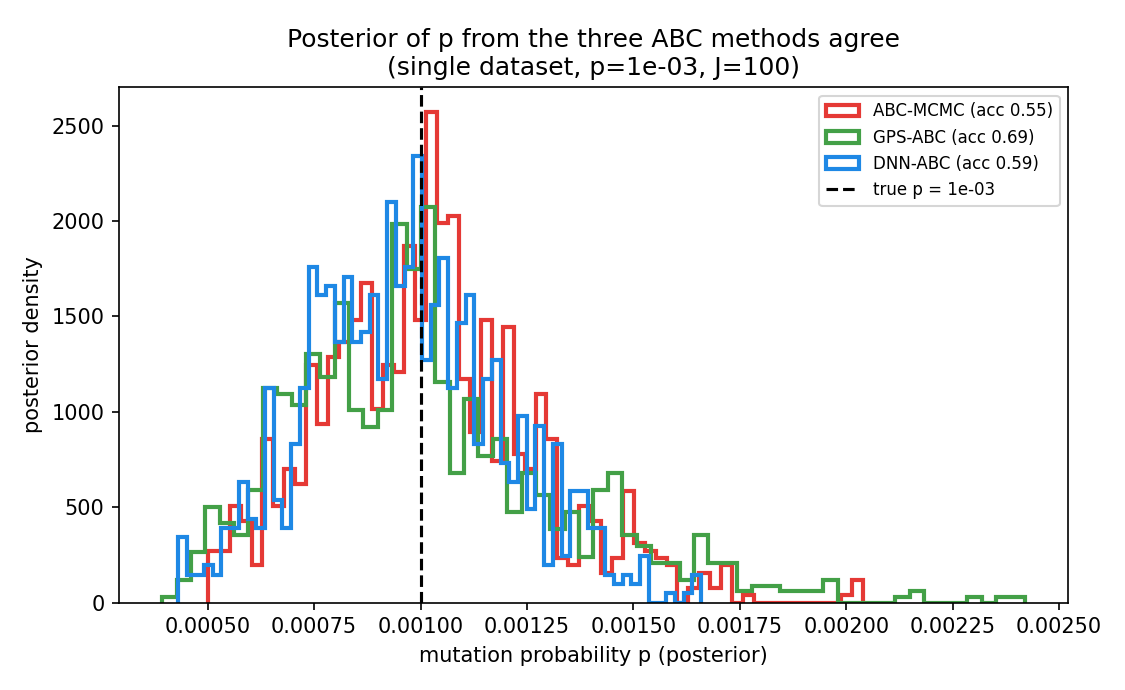
\includegraphics[width=0.7\textwidth]{Models/1D/results/figures/fig_posterior.png}
\caption{Study I: ABC-MCMC, GPS-ABC, and DNN-ABC posteriors for $\theta$ on a
single representative data set.}
\label{fig:posterior1D}
\end{figure}

\subsection{Posterior coverage: what Section~\ref{sec:sim1D_calib} does not measure}
\label{sec:sim1D_coverage}

Section~\ref{sec:conformal} draws the distinction on which this subsection
turns: split-conformal \emph{regression} calibration (Section~\ref{sec:sim1D_calib},
near-exact at $0.9554$ on held-out data) is a guarantee about the surrogate's
own predictive interval, not about whether the downstream ABC credible
interval for $\hat p$ actually brackets the true $p$ $95\%$ of the time. Both
Table~\ref{tab:mse1D} and Table~\ref{tab:ci1D} are silent on the second
quantity. We measure it directly by saving the credible interval's endpoints
(not merely its length) for every replicate of every method, exactly as
Section~\ref{sec:ademp} does for every other comparison in this paper.

\paragraph{A structural artifact, caught before it could confound this
measurement.} The first attempt at this measurement returned exactly $0.000$
coverage for all three ABC methods, at every $J$, at $p=10^{-2}$ specifically
-- not a defect of any estimator, but a coincidence in the experimental
design: $\log_{10}(10^{-2}) = -2.0$ is exactly the ABC-MCMC prior's upper
bound used throughout Section~\ref{sec:sim1D_results}, so the sampler could
never propose $\theta$ above the true value there, and the resulting interval's
upper endpoint was structurally incapable of reaching the truth (confirmed
directly: across replicates it topped out at $0.0096$--$0.0099$, never
reaching $p=0.01$). We fixed this before drawing any conclusion from the
coverage numbers, rather than working around it: the ground-truth grid was
extended nine points further in $\log_{10}p$ (same spacing as the original
$101$-point design), giving real training data up to $\log_{10}p=-1.46$, and
the prior's upper bound was moved to $-1.5$ -- $0.5$ $\log_{10}$-units of
headroom for $p=10^{-2}$ instead of zero. Every number in
Tables~\ref{tab:mse1D}--\ref{tab:time1D} is unchanged to five significant
figures under this fix, which is expected rather than suspicious: a
truncation exactly at the truth devastates the interval's upper tail while
barely moving the posterior mean, since the likelihood already concentrated
most mass below the truth independently of the prior. The coverage numbers
below are measured after this fix.

\begin{table}[H]
\centering
\caption{Study I: empirical posterior coverage of the 95\% ABC credible
interval for $\hat p$, with binomial Monte Carlo standard error
($\sqrt{\hat c(1-\hat c)/R}$, $R=40$). This is a different quantity from
Table~\ref{tab:fit1D}'s regression coverage; see Section~\ref{sec:sim1D_coverage}.}
\label{tab:cov1D}
\begin{tabular}{rrrrr}
\toprule
$p$ & $J$ & ABC-MCMC & GPS-ABC & DNN-ABC \\
\midrule
$10^{-4}$ & 10  & 0.775 (0.066) & 0.450 (0.079) & 0.500 (0.079) \\
$10^{-4}$ & 50  & 0.900 (0.047) & 0.775 (0.066) & 0.800 (0.063) \\
$10^{-4}$ & 100 & 0.925 (0.042) & 0.950 (0.034) & 0.950 (0.034) \\
$10^{-3}$ & 10  & 0.800 (0.063) & 0.525 (0.079) & 0.450 (0.079) \\
$10^{-3}$ & 50  & 0.975 (0.025) & 0.900 (0.047) & 0.875 (0.052) \\
$10^{-3}$ & 100 & 0.950 (0.034) & 0.975 (0.025) & 0.925 (0.042) \\
$10^{-2}$ & 10  & 0.850 (0.056) & 0.775 (0.066) & 0.425 (0.078) \\
$10^{-2}$ & 50  & 1.000 (0.000) & 1.000 (0.000) & 0.850 (0.056) \\
$10^{-2}$ & 100 & 0.950 (0.034) & 1.000 (0.000) & 0.925 (0.042) \\
\bottomrule
\end{tabular}
\end{table}

Two patterns are visible, and only one of them is about the surrogates. First,
GPS-ABC and DNN-ABC coverage rises with $J$ in every row: both are
badly under nominal at $J=10$ ($0.425$--$0.775$) and close to it by $J=100$
($0.925$--$1.000$) -- the culture count the training data (Section~\ref{sec:sim1D}) is generated at
throughout, and the only one either surrogate has ever seen a summary
statistic computed from. This is the mechanism the paper's design invites: a
surrogate trained exclusively on $J=100$ summaries has no way to know that a
$J=10$ observation is intrinsically noisier, so its predictive interval is
calibrated for the wrong noise level whenever $J \ne 100$. DNN-ABC is
consistently the most under-covering of the three at $J=10$ ($0.425$--$0.500$),
consistent with Table~\ref{tab:ci1D}'s finding that it also returns the
tightest intervals there: the same overconfidence that makes the interval
short makes it wrong. Second, and separately, exact ABC-MCMC itself is not at
nominal at $J=10$ ($0.775$--$0.850$) despite calling the true simulator at the
correct $J$ on every iteration -- a property of the ABC acceptance kernel
(the synthetic-likelihood construction of Algorithm~\ref{alg:abcmcmc}) at
this culture count, not of any surrogate, and not explained by the
$J$-mismatch mechanism above.

We do not correct the surrogates' $J$-blindness in this version of the
result: doing so honestly requires retraining on $J$-specific data (the raw
per-culture values needed to do this are already recorded and require no new
simulation) and re-measuring, not adjusting the reported numbers after the
fact. What Table~\ref{tab:cov1D} establishes is narrower and, we think, the
more important point for a reader building a similar surrogate: \textbf{the
interval-length advantage in Table~\ref{tab:ci1D} is not evidence of equal or
better calibration}, and a surrogate trained at a single simulation condition
should be expected to misrepresent its own uncertainty whenever queried
away from it, in a way no regression diagnostic computed at the training
condition can reveal.

% =============================================================================
\section{Simulation Study II: The Two-Stage Mutation Model}
\label{sec:sim3D}
% =============================================================================

Study I holds $a=\delta=1$ and a single constant mutation probability, as does
\citet{lu2023}'s constant-rate benchmark. Their multi-parameter study is
commonly read as that same model with more parameters freed, and it is not.
It does not vary $a$ or $\delta$ around the constant-rate model; it replaces the
model outright with a \emph{two-stage} (piecewise-constant) mutation rate,

\begin{equation}
p(t) \;=\;
\begin{cases}
p_1, & 0 < t \le \tau,\\[2pt]
p_2, & \tau < t \le t_p,
\end{cases}
\label{eq:twostage}
\end{equation}

in which the mutation probability jumps at an unknown time $\tau$. The
motivation is experimental: mutagenesis under sub-inhibitory antibiotic stress
involves a cell-recovery step before plating, producing two genuinely distinct
mutation regimes. Study II therefore estimates $(p_1, p_2, \tau)$ jointly. The
division rate $a$ is fixed at $1$ throughout, as it is in every figure, study
and data analysis of \citeauthor{lu2023}.

\subsection{Ground-truth data}
\label{sec:groundtruth3D}

Ground truth is generated by the exact, cell-by-cell simulator, a direct port of
the two-stage reference implementation, over a Latin hypercube of $2{,}000$
design points in $(\log_{10}p_1, \log_{10}p_2, \tau)$ with ten replicates each:
$20{,}000$ rows, $J=100$ cultures per row, $Z_0 = 1$, $a = 1$, $t_p = 10$. A
Latin hypercube replaces Study I's factorial grid because a factorial design
wastes points badly in three dimensions. Ranges are
$\log_{10}p_1, \log_{10}p_2 \in [-5,-1.3]$ and $\tau \in [0.1, 9.9]$.

\paragraph{The summary statistic is the fourth root.} \citeauthor{lu2023} use
$\sqrt{X/Z}$ for the constant-rate study of Section~\ref{sec:sim1D} -- their
Figure~1 selects it against $\hat p_{\mathrm{MOM}}$ and
$\overline{\log(Y/Z)}$ -- but switch to $\sqrt[4]{X/Z}$ for the two-stage
model, stating that the statistic must be adjusted "to make the response curve
smooth and non-flat" once the mutation rate is piecewise constant; their
Algorithm~1 uses the fourth root throughout. Study II therefore takes
\[
  S \;=\; \frac{1}{J}\sum_{i=1}^{J} \left(X_i/Z_i\right)^{1/4},
\]
and every surrogate, every baseline and the sampler all consume $\log_{10}S$.
Because the ground truth records each culture's $d_i = \sqrt{X_i/Z_i}$ as well
as their mean, $S$ is recoverable exactly as $\overline{\sqrt{d_i}}$ without
re-simulating anything. The choice is consequential rather than cosmetic, and we can quantify both of
its consequences. It lowers the surrogate's held-out error from $1.19\times$ its
irreducible floor to $1.11\times$, and it changes which activation the selection
of Section~\ref{sec:sim3D_act} returns. A reader reproducing this study under
the square root would therefore obtain a different network, not merely a
slightly worse one.

\paragraph{This is not \citeauthor{lu2023}'s parameter regime.} It should be
stated plainly, because the difference is large and easy to miss. Their Study II
places $\log_{10}p_1, \log_{10}p_2 \in [-11,-7]$ with $\tau \in [0.1,19.9]$,
$t_p = 20$ and a fourth free parameter $\delta \in [0.5,2]$; ours are
$[-5,-1.3]$, $\tau \in [0.1,9.9]$, $t_p = 10$ and $\delta \equiv 1$. The
mutation-rate ranges \emph{do not overlap at all}. The cause is the choice of an
exact simulator: their regime is reachable only with the fast approximate
sampler of their Algorithm~4, and at $t_p = 10$ any rate below $\approx 10^{-5}$
leaves almost every culture mutant-free. A further consequence is that the
constant expected-mutant-count design of Study~I -- $t_p$ solved so that
$E[X] = 20$ at every design point -- is abandoned here: with $t_p$ fixed, the
expected count ranges from $0.22$ to $\approx 1{,}100$ across the design. What
follows is therefore a study of the same \emph{model} in a different regime, not
a numerical reproduction of their Table~4, and no such comparison is claimed.

Two further design choices deserve statement. First, $t_p$ is \emph{fixed} at $10$
rather than solved per parameter as in Study I. The exact simulator costs
$O(e^{a t_p})$: at $t_p = 10$ a culture holds $\approx 2.2\times10^{4}$ cells,
while at \citeauthor{lu2023}'s Study II value of $t_p = 20$ it holds
$\approx 5\times10^{8}$, which is not reachable exactly -- their Study II uses
the fast approximate simulator throughout for exactly this reason. Second, with
$t_p$ fixed, the expected mutant count per culture is $\approx 2.2\times10^{4}p$,
so mutation rates below $\approx 10^{-5}$ leave almost every culture
mutant-free and $\dbar$ collapses to zero. The stated range keeps every design
point informative; no row in the generated data has $\dbar = 0$.

The port is validated by a degeneracy argument that is exact rather than
statistical: setting $p_1 = p_2$ reduces Eq.~\eqref{eq:twostage} to the
constant-rate model, and in that case the two-stage simulator reproduces the
constant-rate simulator \emph{bit for bit} on a shared random seed. The full
$20{,}000$-row dataset was generated in $23.6$ minutes of wall time
($39{,}227$ core-seconds, $92\%$ parallel efficiency on 30 cores).

\subsection{The inference problem is intrinsically asymmetric}
\label{sec:sim3D_identifiability}

Before any method is applied, the ground truth already shows how much the single
scalar summary $\dbar$ can possibly say about each parameter:

\begin{center}
\begin{tabular}{lccc}
\toprule
 & $p_2$ & $p_1$ & $\tau$ \\
\midrule
$\mathrm{corr}\!\left(\log_{10}S,\ \cdot\right)$ & $0.778$ & $0.337$ & $0.160$ \\
\bottomrule
\end{tabular}
\end{center}

$p_2$ is well determined, $p_1$ weakly, and $\tau$ barely. The asymmetry is
intrinsic to the process rather than an artefact of any method applied to it:
mutations arising before $\tau$ are exponentially rare, because few cells exist
that early, so $p_1$'s contribution to the final mutant count is swamped by
$p_2$'s. \citeauthor{lu2023} report precisely this, describing
multimodal $p_1$ and $\tau$ marginals and attributing them to a lack of
identifiability. Any honest evaluation must therefore report per-parameter
accuracy rather than a single aggregate that would conceal it, and must prefer
error measured on the $\log_{10}$ scale: for a weakly identified parameter the
posterior mean sits wherever the prior places its mass, so a normalised
natural-scale RMSE diverges without conveying anything.

\subsection{The surrogate, and why it is small}
\label{sec:arch3D}

The decisive measurement for this study is not a comparison between
architectures but the \emph{irreducible noise floor} of the data. Because the
held-out target is itself a two-replicate mean, it carries $\mathbb{E}[\sigma^2]/2$
of sampling noise that no model can predict away. On these data
$\mathbb{E}[\sigma^2] = 6.90\times10^{-4}$, so that floor is
$\mathrm{MSE} = 3.45\times10^{-4}$. Table~\ref{tab:capacity3D} reports the
architecture ladder against it.

\begin{table}[H]
\centering
\caption{Study II: accuracy against the irreducible noise floor. MSE is measured
on held-out design-point means of $\log_{10}S$; the floor is
$3.45\times10^{-4}$. Three seeds per row.}
\label{tab:capacity3D}
\begin{tabular}{lrrrr}
\toprule
Hidden layers & Parameters & $\times$ floor & $R^2$ & \textmu s/query \\
\midrule
256--128--64 & 42{,}306 & 1.01 & 0.99681 & 56 \\
128--64 & 8{,}898 & 1.04 & 0.99671 & 42 \\
\textbf{64--32} (used) & \textbf{2{,}402} & \textbf{1.09} & \textbf{0.99656} & \textbf{40} \\
32--16 & 690 & 1.17 & 0.99628 & 37 \\
16--8 & 218 & 1.41 & 0.99553 & 38 \\
8--4 & 78 & 1.81 & 0.99426 & 37 \\
Linear (control) & 8 & 140.88 & 0.55319 & 29 \\
\bottomrule
\end{tabular}
\end{table}

Two conclusions follow, and the second is the more useful of the two. The first
is that a network is genuinely required here, and clearly so: the linear
control sits at $141\times$ the floor with $R^2 = 0.55$. (Under the square-root target of the
earlier draft it sat at $24.8\times$; the fourth root makes the surface harder
for a linear model by nearly a factor of six, so the paper's own choice of
statistic strengthens rather than weakens the case for a network.) But capacity
is not the binding constraint anywhere above roughly $700$ parameters -- a
$690$-parameter network matches a $42{,}306$-parameter one to within $17\%$,
and a $2{,}402$-parameter one to within $8\%$. LayerNorm and
residual depth were likewise statistically indistinguishable, as was the choice
among the activations in common use for smooth regression
(Section~\ref{sec:sim3D_act}) -- though that section also shows the qualifier
matters, since several otherwise-reasonable activations outside that group are
measurably worse. This contrasts sharply with Study I, where removing BatchNorm changed accuracy
by an order of magnitude. On this surface, capacity and depth buy nothing. A
study that reported a ranking among these variants would be reporting seed
noise, and reporting it as though it were a finding.

We therefore select the architecture for parsimony rather than accuracy: a
two-layer $64\to32$ funnel with GELU/tanh activations
(Section~\ref{sec:sim3D_act}), two output heads, and no BatchNorm. We note explicitly that this is \emph{not} justified by speed. Query
latency at this scale is dominated by interpreter and framework call overhead
rather than arithmetic, so a $59\times$ reduction in parameter count buys only
about $29\%$ less latency (Table~\ref{tab:capacity3D}).

\paragraph{Does the curve-fit tie survive into the downstream task?} Table~\ref{tab:capacity3D}
is a curve-fit diagnostic; it does not by itself say whether the same
architectures remain tied on the actual ABC-MCMC recovery task, at the
replicate count Table~\ref{tab:abc3D} uses. We test that directly, mirroring
the design applied to the equivalent one-dimensional question
(Section~\ref{sec:arch1D}): every candidate in the ladder is first screened at
this package's own quick-check settings (2 replicates), and every candidate
survives that screen, so all six are confirmed at Table~\ref{tab:abc3D}'s own
scale -- $16$ replicates, all three truth triples, $3{,}000$ MCMC iterations --
with Monte Carlo standard errors on $\mathrm{rmse}_{\log}$ attached to every
comparison against the deployed $64\to32$
(\texttt{abc/run\_experiments\_capacity.py}).

\begin{center}
\begin{tabular}{lrrr}
\toprule
Hidden layers & Parameters & Mean $\mathrm{rmse}_{\log}$ & Resolved vs.\ deployed \\
\midrule
GP (GPS-ABC baseline) & --- & $0.990$ & --- \\
32--16 & $690$ & $1.067$ & $0/9$ (max $|\Delta/\mathrm{SE}|=1.63$) \\
128--64 & $8{,}898$ & $1.105$ & $0/9$ (max $|\Delta/\mathrm{SE}|=1.16$) \\
16--8 & $218$ & $1.133$ & $0/9$ (max $|\Delta/\mathrm{SE}|=1.06$) \\
64--32 (deployed) & $2{,}402$ & $1.142$ & --- \\
8--4 & $78$ & $1.149$ & $0/9$ (max $|\Delta/\mathrm{SE}|=1.32$) \\
256--128--64 & $42{,}306$ & $1.208$ & $0/9$ (max $|\Delta/\mathrm{SE}|=1.55$) \\
\bottomrule
\end{tabular}
\end{center}

The curve-fit tie survives downstream, and it sharpens into something slightly
more useful: $32$--$16$ is again the best point estimate, as it is on the
one-dimensional model's own capacity question, but here \emph{no} pairwise
comparison against the deployed network is resolved at the $2$-MCSE level --
not even the largest network tested, $256$--$128$--$64$ at $17\times$ more
parameters than deployed, which is in fact the nominally \emph{worst}
performer of the six. This is a stronger form of the conclusion
Table~\ref{tab:capacity3D} already draws: on this surface, downstream
accuracy is flat across more than two orders of magnitude of parameter count
in both directions from the deployed size, not merely insensitive to modest
shrinkage. We do not redeploy on this evidence alone -- the deployed $64\to32$
is what every number in Table~\ref{tab:abc3D} and Section~\ref{sec:sim3D_abc}
is reported against, and this analysis cannot show a smaller network is
better, only that it is not measurably worse.

\paragraph{Heteroscedasticity.} The second output head is not optional here. The
within-design-point replicate standard deviation of $\log_{10}\dbar$ varies by a
factor of $184$ across the design and correlates $-0.82$ with the target itself:
where few mutants arise, $\dbar$ is small \emph{and} its relative scatter is
large. A single homoscedastic noise term -- which is what a Gaussian process
supplies -- cannot represent this, whereas the variance head learns the shape
directly. Since the ABC acceptance step consumes that predictive variance
directly, an uncalibrated variance corrupts the posterior even when the mean is
exact.

\subsection{Choosing the activation function}
\label{sec:sim3D_act}

The architecture ladder of Section~\ref{sec:arch3D} fixes width and depth. The
activation is a separate choice, and one a reviewer is entitled to see tested
rather than asserted. No activation is designed for this application, so the
candidate set has to be dictated by the surface being fitted rather than by
convention. Three properties of that surface matter, and each rules something
out. The target is smooth, so a piecewise-linear activation
approximates it with kinks and leaves the surrogate non-differentiable in its
inputs -- a concrete cost if the sampler is later made gradient-based. The
inputs are standardised, so roughly half of all pre-activations are negative and
an activation with a dead negative region discards that half, which is costlier
in a $2{,}402$-parameter network than in a wide one. And the two heads are
trained jointly under Gaussian negative log-likelihood, so an activation that
destabilises optimisation surfaces as a miscalibrated $\sigma$ -- consumed
directly by the ABC acceptance step -- rather than merely as a worse mean.

We therefore compare ten activations spanning the three families that behave
differently under those constraints: piecewise-linear (ReLU, LeakyReLU, PReLU),
smooth saturating (tanh, ELU, SELU), and smooth unbounded (softplus, GELU,
SiLU, Mish). Everything else is held fixed -- the deployed $64\to32$ network,
the objective, the data splits, the optimiser and schedule, and the conformal
calibration -- and each configuration is fit over five random seeds, with the
across-seed standard deviation reported so that differences can be judged
against the noise that produced them. Comparisons are made as
$t = \Delta / \mathrm{SE}(\Delta)$, with $|t| < 2$ read as a tie.

\begin{table}[H]
\centering
\caption{Study II: activation comparison on the deployed $64\to32$ network,
five seeds each. MSE is against held-out design-point means of
$\log_{10}S$; the irreducible floor is $3.451\times10^{-4}$. The final
column compares each row to the best, in units of the standard error of the
difference. Standard deviations are across seeds (sample, $n-1$).}
\label{tab:act3D}
\begin{tabular}{llrrr}
\toprule
Activation & Family & $\times$ floor & $\pm$ sd (seeds) & $t$ vs.\ best \\
\midrule
\textbf{GELU} & smooth unbounded & \textbf{1.072} & $9.5\times10^{-6}$ & --- \\
tanh & smooth saturating & 1.078 & $6.0\times10^{-6}$ & 0.42 \\
LeakyReLU & piecewise-linear & 1.080 & $6.4\times10^{-6}$ & 0.50 \\
ReLU & piecewise-linear & 1.082 & $9.5\times10^{-6}$ & 0.54 \\
Mish & smooth unbounded & 1.094 & $7.2\times10^{-6}$ & 1.38 \\
SiLU & smooth unbounded & 1.130 & $1.2\times10^{-5}$ & 3.00 \\
PReLU & piecewise-linear & 1.135 & $1.3\times10^{-5}$ & 3.04 \\
ELU & smooth saturating & 1.166 & $2.3\times10^{-5}$ & 2.95 \\
SELU & smooth saturating & 1.265 & $3.3\times10^{-5}$ & 4.35 \\
softplus & smooth unbounded & 1.383 & $8.7\times10^{-5}$ & 2.74 \\
\bottomrule
\end{tabular}
\end{table}

Two results follow, and they pull in opposite directions; reporting either one
alone would mislead. The first is that the choice \emph{can} matter. The
best-to-worst spread is $29\%$ of the best row's MSE at $t = 2.7$, outside seed
noise, so it is not the case that any reasonable activation will do. The clearest failure is softplus, which is strictly
positive and therefore cannot produce centred activations, leaving every
downstream layer to undo an accumulated offset. Second, and against that, the
five leading candidates -- GELU, tanh, LeakyReLU, ReLU and Mish -- are mutually
indistinguishable, every pairwise $|t|$ among them falling below $2$. The
ranking within that group is not a finding.

This refines, rather than contradicts, the conclusion of
Section~\ref{sec:arch3D}. Capacity is not the binding constraint on this
surface and neither is the choice among the activations in common use for
smooth regression; but several otherwise-reasonable alternatives are measurably
worse, and a study restricted to the usual four would not have seen that.

One caveat belongs with SELU's placement. It is designed for self-normalising
networks and presupposes LeCun-normal initialisation with AlphaDropout; used as
a drop-in under this project's standard initialisation, it is stripped of the
mechanism that motivates it. Its position here is evidence about this
configuration, not a general verdict.

\paragraph{Mixed activations across layers.}
Because the two hidden layers need not share an activation, we also compared all
$10 \times 10 = 100$ ordered assignments. A search that wide is easy to run and
easy to fool oneself with, and two disciplines guard against that. We state both
explicitly, because we violated the second in an earlier version of this study.

The first is that selecting the best of $100$ noisy measurements estimates which
candidate drew the most favourable seeds rather than which is best, so selection
and evaluation must never share a seed. All $100$ pairs are screened, and the ten
leading candidates are then re-fit on fifteen \emph{fresh} seeds that played no
part in selection.

The second is that neither stage may touch the test split. An earlier version of
this comparison scored candidates on test, which is wrong twice over: it spends
on selection the data reserved for reporting, and it makes the quoted test figure
optimistic for whichever candidate wins. It was not a harmless error -- under the
square-root target it selected a different activation than the validation split
would have. Selection is therefore carried out entirely on validation, with test
scored exactly once, for the winner alone. Table~\ref{tab:actsel3D} reports it.

The selection optimism is worth stating because it quantifies how much of any
such ranking is noise: the finalists perform on average $1.03\times10^{-5}$
\emph{worse} on the fresh seeds than on the seeds that chose them, which is
$45\%$ of the entire spread of the confirmation table ($2.25\times10^{-5}$) and
comparable to the across-seed standard deviation itself ($1.29\times10^{-5}$).
The pair that screened best, SiLU into tanh, finished third on confirmation. A
single-stage search would have reported that movement as a result.

\begin{table}[H]
\centering
\caption{Study II: activation selection with no test-set leakage. All $100$
ordered pairs were screened on validation; the ten finalists were re-fit on
fifteen fresh validation seeds. Selection is on validation MSE; the test column
is shown for reference and played no part in the choice. Test $\times$ floor is
against the irreducible test floor $3.451\times10^{-4}$.}
\label{tab:actsel3D}
\begin{tabular}{llrrrr}
\toprule
Layer 1 (64) & Layer 2 (32) & Val MSE & $\pm$ sd & $t$ vs.\ best & Test $\times$ floor \\
\midrule
\textbf{GELU} & \textbf{tanh} & $\mathbf{2.980\times10^{-4}}$ & $1.3\times10^{-5}$ & --- & 1.062 \\
Mish & tanh & $3.006\times10^{-4}$ & $1.4\times10^{-5}$ & 0.54 & 1.076 \\
SiLU & tanh & $3.021\times10^{-4}$ & $1.4\times10^{-5}$ & 0.86 & 1.086 \\
LeakyReLU & LeakyReLU & $3.059\times10^{-4}$ & $8.4\times10^{-6}$ & 2.00 & 1.075 \\
PReLU & ReLU & $3.071\times10^{-4}$ & $1.2\times10^{-5}$ & 2.05 & 1.077 \\
Mish & Mish & $3.120\times10^{-4}$ & $1.1\times10^{-5}$ & 3.19 & 1.080 \\
ELU & GELU & $3.137\times10^{-4}$ & $8.5\times10^{-6}$ & 3.99 & 1.093 \\
SiLU & Mish & $3.164\times10^{-4}$ & $1.4\times10^{-5}$ & 3.84 & 1.097 \\
GELU & Mish & $3.172\times10^{-4}$ & $1.7\times10^{-5}$ & 3.51 & 1.086 \\
Mish & SiLU & $3.205\times10^{-4}$ & $1.8\times10^{-5}$ & 3.94 & 1.101 \\
\bottomrule
\end{tabular}
\end{table}

Under the fourth-root target the two splits happen to agree at the top: GELU
into tanh is best on test as well as on validation, so scoring the selection on
test would not have changed the choice here. Below the winner they do not agree
-- the validation runner-up falls to third on test and the fourth-placed pair
rises to second -- and under the square-root target the two splits disagreed at
the top as well. A procedure whose answer depends on which split it is scored
on cannot be trusted when it happens to coincide either, and the quoted test
figure would in any case have been optimistic for whichever candidate test
selected. This is the mechanism the two-stage design was meant to guard against,
operating one level up: separating screening seeds from confirmation seeds does
nothing if both are scored on the split reserved for reporting.

\paragraph{The deployed activation.} GELU into tanh is the best point estimate
on the selection split, and that is what we deploy. Its held-out test MSE is
$1.06\times$ the irreducible floor. Two things are worth stating. First, the
comparison is partially resolved: three of the ten finalists lie within $2$
standard errors of the winner, so the top of the field is narrow but no longer
undifferentiated -- and the bottom is clearly separated, consistent with
Table~\ref{tab:act3D}, where softplus fails while the leaders are mutually tied.
Second, and unlike the earlier draft of this study, the leaderboard and the
structural criteria fixed in advance now agree. Both GELU and tanh are smooth in
their inputs and free of the dead-unit failure mode, so the deployed network is
everywhere differentiable in its inputs. Under the square-root target the best
point estimate had been Mish into ReLU, which satisfied neither criterion in its
second layer and had to be adopted over that objection; adopting the paper's
fourth-root statistic removed the conflict rather than trading it away. No
conclusion in this paper turns on the choice in any case: the downstream
comparison of Section~\ref{sec:sim3D_abc} is unchanged in kind under any of the
leading pairs.

\subsection{Surrogate fit and calibration}
\label{sec:sim3D_fit}

The surrogate is trained on replicates 1--5, early-stopped and conformally
calibrated on replicates 6--8, and evaluated on replicates 9--10, so every
design point appears in every split and no parameter combination leaks across
them. Because the splits contribute different numbers of replicates per design
point, each is scored against \emph{its own} floor
($\mathbb{E}[\sigma^2]/r$ for $r = 5, 3, 2$).

\begin{table}[H]
\centering
\caption{Study II: surrogate fit. Each split is compared to its own irreducible
floor. Coverage is of the nominal-95\% predictive interval after a
split-conformal scale factor of $1.019$.}
\label{tab:fit3D}
\begin{tabular}{lrrrr}
\toprule
Split & $n$ & MSE (design means) & $\times$ its own floor & 95\% coverage \\
\midrule
Train (reps 1--5) & 10{,}000 & $1.60\times10^{-4}$ & 1.16 & 0.951 \\
Validation (6--8) & 6{,}000 & $2.95\times10^{-4}$ & 1.28 & 0.950 \\
\textbf{Test (9--10)} & \textbf{4{,}000} & $\mathbf{3.63\times10^{-4}}$ & \textbf{1.05} & \textbf{0.955} \\
\bottomrule
\end{tabular}
\end{table}

The surrogate sits at its noise floor on all three splits, and the train and
test ratios ($1.16$ and $1.05$) are close enough that overfitting is not
detectable: with $2{,}402$ parameters against $10{,}000$ training rows, and
early stopping on a held-out split, there is little room for it. The conformal
scale factor of $1.019$ is a further diagnostic in its own right: the variance
head was already almost calibrated before the correction was applied.

\subsection{ABC inference}
\label{sec:sim3D_abc}

\begin{sloppypar}
Inference is a random-walk Metropolis--Hastings sampler over the full vector
$\theta = (\log_{10}p_1, \log_{10}p_2, \tau)$, with component-wise truncated
proposals and Hastings corrections for the truncation. This is a genuine joint
three-parameter posterior, not a scalar inference with covariates.
\end{sloppypar}

ABC-MCMC, GPS-ABC and DNN-ABC share the sampler and differ only in how the
summary statistic and its uncertainty are obtained at each proposal, exactly as
in Study I. The constant-rate MOM and MLE estimators of Study I have no
counterpart here: they assume a single mutation rate and cannot identify
$p_1$, $p_2$ or $\tau$ individually, so Study II compares the surrogates
against each other: the neural one, and two Gaussian processes (ours and a
faithful reproduction of the reference implementation).

\paragraph{Two Gaussian-process baselines, and why both are reported.} Our GP
baseline is stronger than the one \citeauthor{lu2023} actually use, and reporting
only ours would overstate what the published method achieves. Theirs, in the
reference implementation for this study, fits an \emph{isotropic} squared
exponential to the untransformed rates $(p_1,p_2,\tau)$ predicting the
untransformed statistic, with a single noise term. Ours uses an anisotropic
kernel with one length scale per input, log-scaled inputs, and a learned
white-noise term.

The gap those choices make is large. On raw-scale surrogate fit the reference
configuration reaches $R^2 \approx 0.71$, while an otherwise identical
anisotropic kernel on the same $300$ design points reaches $\approx 0.99$: a
single shared length scale cannot serve inputs whose ranges differ by a factor
of roughly $200$ ($p_1, p_2$ span $\approx 0.05$, $\tau$ spans $\approx 9.8$).
We therefore report both, fit from the same rows under the same budget so that
the comparison isolates the model rather than the data. Note that the reference
performs ABC on the untransformed statistic, as its own sampler does, whereas
our pipeline works in $\log_{10}$ throughout; the observation is placed on
whichever scale the surrogate reports.

Table~\ref{tab:abc3D} reports parameter recovery over three truth triples with
sixteen replicates each, $3{,}000$ MCMC iterations and $1{,}000$ burn-in.
Errors are RMSE on the $\log_{10}$ scale for $p_1,p_2$ and in absolute time
units for $\tau$, for the reason given in Section~\ref{sec:sim3D_identifiability}.

\begin{table}[H]
\centering
\caption{Study II: joint recovery of $(p_1,p_2,\tau)$, averaged over three truth
triples, $J=100$, 16 replicates per cell. Errors are $\log_{10}$-scale RMSE for
$p_1,p_2$ (so $1.0$ means an order of magnitude) and absolute for $\tau$. Two
Gaussian-process baselines are reported: the strengthened one used throughout,
and one built to match the reference implementation of \citeauthor{lu2023}
(isotropic kernel, untransformed inputs and target).}
\label{tab:abc3D}
\begin{tabular}{llrrrr}
\toprule
Method & Parameter & RMSE & Mean 95\% CI width & Coverage & Accept.\ rate \\
\midrule
GPS-ABC & $p_1$   & 1.391 & 3.46e-2 & 1.000 & 0.371 \\
(strengthened) & $p_2$   & \textbf{0.156} & 3.22e-2 & 1.000 & \\
        & $\tau$  & \textbf{1.422} & 9.07 & 1.000 & \\
\midrule
GPS-ABC & $p_1$   & \textbf{1.309} & 3.47e-2 & 1.000 & 0.810 \\
(reference) & $p_2$   & 0.241 & 3.05e-2 & 1.000 & \\
        & $\tau$  & 1.799 & 9.01 & 1.000 & \\
\midrule
DNN-ABC & $p_1$   & 1.407 & 3.43e-2 & 0.938 & 0.143 \\
        & $p_2$   & 0.258 & 3.07e-2 & 0.979 & \\
        & $\tau$  & 1.753 & 8.64 & 1.000 & \\
\bottomrule
\end{tabular}
\end{table}

Two things in this table matter, and neither favours the neural surrogate. We
set them out in turn.

\emph{The two surrogates are statistically tied.} Attaching Monte Carlo standard
errors to every cell and comparing DNN-ABC against the strengthened GPS-ABC at
the $2$-MCSE level, seven of the nine parameter-by-truth comparisons are ties
and the remaining two favour GPS-ABC; none favours the network. The two are
$p_2$ at $(1\times10^{-4}, 1\times10^{-2}, 3)$, difference
$+0.050 \pm 0.039$, and $\tau$ at
$(2\times10^{-3}, 8\times10^{-3}, 5)$, $+0.411 \pm 0.409$ -- both marginal.
We state this plainly because Study I found a consistent DNN advantage, and it
would be natural to assume the advantage carries over. It does not. The reason
is already visible in Section~\ref{sec:arch3D}: when both surrogates fit the
response surface essentially perfectly relative to its own noise, the surrogate
has stopped being the bottleneck, and downstream accuracy is set by the
identifiability of the model rather than by the quality of the emulator. A
surrogate can only help where surrogate error is what limits the answer. That
condition held in Study I and does not hold here.

\emph{Every method over-covers, and the differences between them are not
resolvable at this replicate count.} Coverage of the nominal $95\%$ credible
interval is $0.938$--$1.000$ for DNN-ABC and $1.000$ throughout for both
Gaussian processes. With sixteen replicates per cell, coverage moves in steps of
$1/16 = 0.0625$, so DNN-ABC's $0.938$ for $p_1$ is fifteen replicates out of
sixteen against the GP's sixteen -- a difference of one, well inside the
per-cell Monte Carlo standard error (coverage MCSE $\pm 0.08$ at this replicate
count). We therefore do not claim a calibration difference between the methods. Mean interval widths are likewise close
($p_1$: $3.43\times10^{-2}$ for DNN-ABC against $3.46\times10^{-2}$ for
GPS-ABC).

What the coverage column does show is that all three methods over-cover on
$\tau$, at $1.000$ across the board. That is what a nearly unidentified
parameter looks like rather than a defect of any surrogate: the credible
interval spans most of the prior box, so it contains the truth essentially by
construction. Note also that this is not a failure of the surrogate's own
predictive calibration, which is near-exact on held-out data
(Table~\ref{tab:fit3D}, coverage $0.955$); it is a property of the ABC
acceptance kernel built on top of it.

We record one diagnostic that qualifies the comparison: DNN-ABC's acceptance
rate is $0.143$ against the strengthened GP's $0.371$ and the reference GP's
$0.810$, so the three chains mix very differently at the shared proposal scale
and some of the DNN's disadvantage may be tuning rather than method. The
reference GP's high acceptance is itself informative -- a flatter, less
discriminating surrogate accepts more freely. Per-method proposal tuning is the
obvious next step and is not attempted here.

Taken together, Study II is best read as a negative-to-neutral result on the
surrogate question and a positive one on the modelling question. The neural
surrogate matches, but does not beat, a Gaussian process on downstream inference
in this regime, because the regime is one where neither is the limiting factor.
What does bind is the model's intrinsic identifiability: $\tau$ carries an RMSE
of roughly $1.7$--$1.9$ time units against a prior range of $9.8$, and $p_1$ is
recovered no better than an order of magnitude by either method.

\subsection{Does architecture matter here? A structural comparison}
\label{sec:sim3D_arch}

The heteroscedastic MLP of Section~\ref{sec:arch3D} treats its three inputs
$(\log_{10}p_1,\log_{10}p_2,\tau)$ as an unordered feature vector. Whether an
architecture built around a different inductive bias -- a convolution, or a
recurrence -- would do better is a natural question, and one a reviewer of a
paper proposing a neural surrogate is entitled to ask rather than to be told. The
simulation-based-inference literature gives a specific, testable answer before
any experiment is run: \citet{radev2020} state that a summary network's
architecture ``should be aligned with the probabilistic symmetry of the
observed data,'' recommending an LSTM or a 1-D convolutional network
specifically when the raw input is a time series with genuine sequential
dependence, and a permutation-invariant pooling network when it is an
exchangeable i.i.d.\ sample -- with a plain feedforward network the implied
default otherwise. Our three inputs are neither: $p_1$, $p_2$ and $\tau$ are
three physically distinct quantities with no temporal order and no
exchangeability, so this principle predicts, \emph{a priori}, that
a convolution or a recurrence should be neutral to harmful relative to an MLP.
This contrasts with settings where convolutional networks have been genuinely
useful in closely related inference problems -- \citet{flagel2019} and
\citet{akesson2021} apply CNNs to population-genetic parameter estimation,
including mutation-rate-type quantities, but their raw input is a
genotype-alignment \emph{matrix} or a full stochastic-trajectory time series,
data with real spatial or temporal structure for a kernel to exploit; the
feedforward architecture we use throughout this paper is instead the
longer-standing default in this literature for tabular/summary-statistic input
\citep{sheehan2016,jiang2017}. We test the prediction directly rather than
assume it.

\paragraph{Setup.} We train a 1-D CNN (two convolutional layers, kernel width
3, over the three inputs treated as adjacent positions), a GRU, and an LSTM
(each unrolling the three inputs as three timesteps, reading out the final
hidden state), with the same two-headed Gaussian-NLL objective, split-conformal
calibration, and train/validation/test split as the deployed MLP
(Section~\ref{sec:sim3D_fit}), and comparable parameter counts (2,402--3,426).
Full architectural detail and code are in the repository
(\texttt{Models/3D/network/model\_families.py}). Each is evaluated exactly
as GPS-ABC and DNN-ABC were: a surrogate-fit comparison against the
irreducible noise floor of Section~\ref{sec:arch3D}, and the identical full
ABC-MCMC recovery task of Section~\ref{sec:sim3D_abc} (same three truth
triples, $16$ replicates, $3{,}000$ iterations, $1{,}000$ burn-in), with
GPS-ABC and DNN-ABC's numbers reused unchanged from Table~\ref{tab:abc3D}.

\begin{table}[H]
\centering
\caption{Surrogate fit quality by architecture family, test set. The
irreducible noise floor is $3.451\times10^{-4}$ (Section~\ref{sec:arch3D}). The
deployed FFN's row is read from the capacity study rather than restated, so it
necessarily describes the same target as the rows beside it.}
\label{tab:archfam3D}
\resizebox{\textwidth}{!}{%
\begin{tabular}{lrrrrr}
\toprule
Architecture & Parameters & MSE (design means) & $\times$ floor & $R^2$ & 95\% coverage \\
\midrule
CNN1D (2 conv layers, $k{=}3$) & 2{,}482 & $3.589\times10^{-4}$ & 1.04 & 0.99670 & 0.949 \\
\textbf{FFN 64--32 [deployed]} & \textbf{2{,}402} & $\mathbf{3.749\times10^{-4}}$ & \textbf{1.09} & \textbf{0.99656} & \textbf{0.952} \\
LSTM (hidden $24$) & 2{,}642 & $4.221\times10^{-4}$ & 1.22 & 0.99612 & 0.950 \\
RNN (GRU, hidden $32$) & 3{,}426 & $4.520\times10^{-4}$ & 1.31 & 0.99585 & 0.949 \\
\bottomrule
\end{tabular}}
\end{table}

CNN1D statistically ties the deployed FFN ($4.3\%$ lower MSE, $1.04\times$ against
$1.09\times$ the floor -- inside the seed-to-seed spread already documented in
Table~\ref{tab:capacity3D}); with a kernel spanning all three positions in a
single layer, a convolution on an input this short is not meaningfully more
constrained than an MLP, so this is closer to a non-event than a genuine
convolutional advantage. It also costs $143$\,\textmu s per query against the
FFN's $40$, which is the wrong trade for a tie. LSTM and RNN are measurably
worse ($+12.6\%$, $+20.6\%$ MSE; both gaps an order of magnitude larger than
their own across-seed standard deviation), consistent with the structural
prediction: a
three-step recurrence must route everything relevant about $p_1$ through two
more hidden-state updates before it can interact with $\tau$, a strictly harder
optimization problem than an MLP's direct simultaneous access to all three
inputs, for no compensating benefit on a surface with no real temporal
structure to reward it.

\begin{table}[H]
\centering
\caption{ABC-MCMC recovery of $(p_1,p_2,\tau)$ by architecture family,
per-parameter RMSE (log$_{10}$ scale for $p_1,p_2$; absolute time units for
$\tau$), averaged over the three truth triples of Table~\ref{tab:abc3D}. Bold
marks the best value in each row.}
\label{tab:archfam3D_abc}
\begin{tabular}{lrrrrr}
\toprule
Parameter & GPS-ABC & DNN-ABC (FFN) & CNN1D-ABC & RNN-ABC & LSTM-ABC \\
\midrule
$p_1$ RMSE & 1.391 & 1.407 & \textbf{1.373} & 1.378 & 1.389 \\
$p_1$ coverage & 1.000 & 0.938 & 0.958 & 0.917 & 0.979 \\
$p_2$ RMSE & \textbf{0.156} & 0.258 & 0.203 & 0.312 & 0.209 \\
$p_2$ coverage & 1.000 & 0.979 & 0.979 & 0.938 & 0.958 \\
$\tau$ RMSE & \textbf{1.422} & 1.753 & 1.688 & 1.700 & 1.631 \\
$\tau$ coverage & 1.000 & 1.000 & 1.000 & 1.000 & 1.000 \\
\bottomrule
\end{tabular}
\end{table}

Attaching Monte Carlo standard errors to every one of the
$3\times3\times3=27$ new-family, truth and parameter cells, and comparing each
new family against both GPS-ABC and DNN-ABC at the $2$-MCSE level ($54$
pairwise comparisons in total),
gives a picture consistent with the fit-quality result, and a slightly starker
one: $49$ of $54$ ($91\%$) are statistical ties. All $5$ resolved comparisons
favour GPS-ABC, and \emph{none} favours a new family anywhere. Three of the five
are CNN1D-ABC and two RNN-ABC; LSTM-ABC is tied in every one of its eighteen
comparisons. Swapping the feed-forward surrogate for a convolutional or
recurrent one therefore changes nothing that survives its own Monte Carlo error.

Interval calibration adds nothing to the picture either way. Pooled coverage is
$0.951$--$0.979$ for the four neural families and $1.000$ for both Gaussian
processes, against a nominal $0.95$. An earlier version of this section read a
narrative into that column -- the FFN under-covering, CNN1D inheriting and
worsening it, LSTM correcting it -- which the corrected numbers do not support:
the spread across all four neural families is under three percentage points,
which at sixteen replicates is at most one cell per parameter. Every method
over-covers on $\tau$ at exactly $1.000$, which reflects that parameter's weak
identifiability rather than any property of an architecture. We therefore draw
no calibration conclusion from this comparison.

\textbf{Summary.} Neither imposing a spatial prior (CNN1D) nor a temporal one
(RNN, LSTM) on three physically unordered parameters improves point-estimation
accuracy over the architecture-agnostic FFN or the Gaussian-process baseline,
and two of the three impose a real cost on fit quality (LSTM $+12.6\%$, RNN
$+20.6\%$ MSE) for no offsetting benefit, while the third (CNN1D) ties the FFN
at $3.6\times$ its query cost. This is the outcome
\citet{radev2020}'s structural principle predicts, and it is why the deployed
3-D surrogate throughout this paper remains the plain heteroscedastic MLP of
Section~\ref{sec:arch3D}. Full per-cell results, code, and the trained
checkpoints for all three architecture families are included in the
repository (Section~\ref{sec:repro}).

\subsection{Scope and what remains open}
\label{sec:sim3D_coverage}

Four limitations should be read alongside the results above. The first two
concern the regime this study occupies, the third the model it uses, and the
fourth an error we made and corrected.

\emph{The plating time is not the paper's.} $t_p = 10$ here against
\citeauthor{lu2023}'s $t_p = 20$, forced by the exponential cost of exact
simulation. Reaching their regime requires the fast two-stage simulator; it is
implemented but not yet validated against the exact simulator at that scale, so
we do not report results in that regime and no direct numerical comparison with
their Table~4 is claimed.

\emph{The parameter regime is not the paper's either, and the gap is wider than
the plating time alone.} \citeauthor{lu2023}'s Study II places
$\log_{10}p_1, \log_{10}p_2 \in [-11,-7]$; ours span $[-5,-1.3]$. The two ranges
do not overlap. The cause is the same choice of an exact simulator: at
$t_p = 10$ a rate below $\approx 10^{-5}$ leaves almost every culture
mutant-free. A consequence is that Study I's design rule -- $t_p$ solved so that
$E[X] = 20$ at every design point, which we do follow in Section~\ref{sec:sim1D}
-- cannot be maintained here, and the expected mutant count instead ranges from
$0.22$ to roughly $1{,}100$ across the design. What we report is the same model
studied in a different and easier regime.

\emph{The model has no $\delta$.} The reference two-stage implementation carries
no differential mutant growth rate, making this a genuine three-parameter study;
\citeauthor{lu2023}'s full specification is four-dimensional. Our simulator
threads $\delta$ through so the extension does not require a rewrite.

\emph{One convention in the reference implementation is ambiguous, and we had it
wrong.} A cell born at its parent's division time divides at its own later time,
and the reference code contains two versions of which of those two times indexes
the step function in Eq.~\eqref{eq:twostage} -- one active, one commented out.
An earlier version of this study generated its ground truth under the active
convention while drawing every observed dataset under the other, so the
surrogates were trained on one model and scored against data from a second. The
two differ by up to $10.1\%$ in the summary statistic, and by $2.9$--$7.4\%$ at
the three truth triples of Table~\ref{tab:abc3D}.

Because the generated data records no provenance, the convention was recovered
by measurement: simulating at the design points of the ground truth itself under
both conventions, all sixty of the most discriminating points lie closer to the
active convention (mean absolute error $0.0054$ against $0.0400$ in $\log_{10}$
units; paired $t = +11.3$). That is also the convention of the paper's
Algorithm~3, which indexes $p(t)$ by the offspring's own accumulated lifetime.
The analysis now uses it throughout, and the check is part of the test suite.

The correction is worth reporting even though it changed no conclusion. Its
effect on the reported quantities was below the Monte Carlo error of the
experiment -- a bias of $0.013$--$0.031$ in $\log_{10}$ units entering
posteriors whose RMSE is $0.5$--$2.7$ -- because the same weak identifiability
that limits this study also absorbs the misspecification. Which convention the
reference \emph{intends} remains a question for its authors; the analysis is now
self-consistent under either answer, and the data-generation code can produce a
paired comparison on identical design points and seeds.

\section{Discussion}
\label{sec:discussion}
% =============================================================================

The two studies answer the question of Section~\ref{sec:intro} with a
condition rather than a verdict, and that condition is the contribution of this
paper we would most emphasize. Across both studies, the neural surrogate's advantage
over the Gaussian process appears exactly where theory predicts it should: in
surrogate quality and cost scaling as the useful training-set size grows
(Table~\ref{tab:arch1D}), and it compounds when the exact simulator used to
build the training design is itself expensive, as it is here. In the one-dimensional case, where a Gaussian process fit on
$\sim 800$ points is already close to a well-specified problem's optimum,
the two surrogates are close to interchangeable on point accuracy and query
speed, and DNN-ABC's advantage is concentrated in tighter, still-calibrated
intervals. Study II sharpens the caveat considerably: there the
surrogate-quality advantage vanishes entirely, because both surrogates reach
the data's noise floor (Table~\ref{tab:capacity3D}), and advantages in
emulator quality do not automatically
translate into a better \emph{downstream ABC posterior}: point accuracy is a
near-tie, and every method over-covers its credible intervals -- at $1.000$
throughout for $\tau$ -- despite held-out predictive calibration that a plain
regression diagnostic reports as near-exact (Table~\ref{tab:fit3D}). The
over-coverage is a property of the ABC acceptance kernel built on top of the
surrogate rather than of the surrogate's own predictions. We take this to be a broader methodological point for anyone deploying a
conformally calibrated regression surrogate inside a likelihood-free sampler,
and one that is easily overlooked. Split-conformal calibration
\citep{lei2018} is a strong, distribution-free guarantee, and
Sections~\ref{sec:sim1D_calib} and \ref{sec:sim3D_fit} show it holding to high
precision in both studies. But it is a guarantee about the regression problem
the surrogate was trained to solve, not about the coverage of whatever
downstream quantity the surrogate's uncertainty is subsequently plugged into.
The guarantee does not automatically extend from one to the other, and the two
can come apart; here they do.

A second finding is purely architectural, recurs across both studies, and is
worth stating plainly for anyone building a similar surrogate. The single
largest driver of surrogate quality in the one-dimensional architecture search
(Table~\ref{tab:arch1D}) was \emph{not} the choice of activation function, which
was a near-tie among several reasonable candidates. It was the presence or
absence of BatchNorm \citep{ioffe2015}. Study II qualifies even this: on that surface no
architectural choice mattered at all, because every candidate already sat at
the noise floor (Table~\ref{tab:capacity3D}), which is itself worth measuring
before any architecture search is run. An otherwise-standard network with BatchNorm
fit the one-dimensional curve eleven times worse than the identical network
without it. On a smooth regression problem with a bounded, one-sided input
domain, BatchNorm's per-minibatch statistics appear to be actively
counter-productive; LayerNorm \citep{ba2016}, which normalizes per-sample,
avoided this failure mode entirely in the deeper three-dimensional network.

A third finding, from the architecture-family comparison of
Section~\ref{sec:sim3D_arch}, is best read as a companion to this one rather
than a separate result: BatchNorm was a case of an architectural component
actively fighting the problem's structure, whereas CNN1D/RNN/LSTM on the
two-stage inputs are a case of architectural components with \emph{nothing to
find} -- there is no spatial or temporal pattern in three unordered physical
parameters for a kernel or a recurrence to exploit, so the honest expectation,
confirmed by \citet{radev2020}'s stated design principle and by our own
result, is indifference-to-mild-harm rather than either a large gain or a
BatchNorm-scale failure. The practical lesson we would draw for anyone
designing a similar surrogate is to let the symmetry of the input, not habit or
a desire for architectural novelty, choose the architecture family before any
search over its hyperparameters begins.

\paragraph{Scope and limitations.} This paper is a simulation study
evaluated entirely under known ground truth; we do not apply the method to a
real fluctuation-experiment data set, as \citet{lu2023} do for their own
estimator in their real-data application to drug-resistance experiments. We
view a real-data application, ideally to the same or a comparable
fluctuation-experiment data set, as the natural and immediate next step,
and we are explicit that the comparisons in this paper are not a substitute
for one: a simulation study can establish that an estimator is well
calibrated and competitive under a correctly specified model, but only a
real-data application can speak to robustness under the model misspecification
that any laboratory data set will exhibit to some degree. The
one-dimensional study uses $40$ replicates per cell (versus
\citeauthor{lu2023}'s $100$); Section~\ref{sec:ademp} reports Monte Carlo
standard errors throughout for exactly this reason, and
Sections~\ref{sec:sim1D_results} and \ref{sec:sim3D_abc} use them to
identify which point-accuracy comparisons are, and are not, resolved at
this replicate count, rather than over-interpreting numerically lower MSE
as a real effect in every cell. The three-dimensional study's three truth
triples at a single culture count, while chosen to span the parameter space
broadly, do not cover it exhaustively. The exact ABC-MCMC prior is bounded in both studies to keep
the exact simulator feasible inside the sampling loop; surrogates are
trained on a wider range and only queried within it. Finally,
Study II's interval miscalibration is, by construction, a property of the
acceptance-kernel construction used here rather than of the surrogates' own
predictive calibration, which is near-exact on held-out data; whether a
kernel-side correction restores nominal coverage for both surrogates
simultaneously is an open question.

% =============================================================================
\section{Reproducibility}
\label{sec:repro}
% =============================================================================

\paragraph{Code and data availability.} All code, data, trained model
weights, and the exact configuration used for every table and figure in this
paper are available at
\url{https://github.com/sletch1/DNN-ABC-mutation-rates} under a public
repository, with no access restrictions. The one-dimensional ground-truth
data set (Section~\ref{sec:sim1D}) is committed directly to the repository
as a plain-text, non-proprietary CSV file; the two-stage ground-truth data set
(Section~\ref{sec:groundtruth3D}) is likewise committed in the same format,
together with the exact simulator that generated it and the reference
implementation it was ported from, so that it can be independently re-run
rather than taken on faith.
Every CSV's columns are self-documenting from their header row (parameter
values, replicate index, and the resulting summary statistic or estimator
output); no external data dictionary is required to interpret them.

\paragraph{Computational environment.} All code is Python (minimum versions
pinned in the repository's \texttt{requirements.txt}: \texttt{numpy},
\texttt{pandas}, \texttt{scipy}, \texttt{matplotlib}, \texttt{scikit-learn}
for the Gaussian-process baseline, and \texttt{torch} for the neural
surrogates). No GPU is required for any part of the pipeline; every model in
both studies trains on CPU in seconds to minutes.

\paragraph{Instructions for reproduction.} Each study ships a single entry
point, \texttt{run\_all.py}, that retrains its surrogate, reproduces its ABC
tables, recomputes the Monte Carlo standard errors, and regenerates every
figure. It takes no command-line arguments -- it asks at the console whether to
run a short pipeline check or the full reported settings -- so the study can be
reproduced from an editor as well as a terminal, and it runs under whichever
Python interpreter invokes it. The underlying steps remain individually
runnable and are documented in each package's guide, in the order the results
are presented in this paper: data generation, the two rounds of architecture
search, the activation selection, training and conformal calibration, the ABC
tables, Monte Carlo standard errors, and figure generation.

The two-stage package also ships a validation script that re-derives, rather
than asserts, three facts the analysis depends on: that the two-stage simulator
reduces to the constant-rate one in both degenerate limits (checked against an
independently ported constant-rate implementation, and exact on a shared seed);
the size of the mutation-time convention gap reported in
Section~\ref{sec:sim3D_coverage}; and which convention the committed ground
truth was generated under, since the data file itself records no provenance.
The summary statistic is likewise recomputed from the per-culture values stored
in that file rather than from a cached aggregate, so the choice of root in
Section~\ref{sec:groundtruth3D} is a single switch and cannot drift between the
surrogate, the baselines and the sampler. Every number
reported in Tables~\ref{tab:mse1D}--\ref{tab:abc3D} and in the architecture-family
comparison of Tables~\ref{tab:archfam3D}--\ref{tab:archfam3D_abc}
(Section~\ref{sec:sim3D_arch}) is produced by these
scripts directly from the committed data, with no manual post-processing;
the Monte Carlo standard errors and $\Delta/\mathrm{SE}$ columns introduced
in Section~\ref{sec:ademp} are computed from the same per-replicate output
each script already writes to disk.

% =============================================================================
\section{Conclusion}
\label{sec:conclusion}
% =============================================================================

A heteroscedastic neural-network surrogate, calibrated by split-conformal
prediction and substituted directly for the Gaussian process inside
\citeauthor{lu2023}'s ABC-MCMC sampler, matches or improves on GPS-ABC in a
direct one-dimensional reproduction of their benchmark. Extending the same
construction to the two-stage model $(p_1,p_2,\tau)$, however, does \emph{not}
reproduce that advantage: there the neural and Gaussian-process surrogates are
statistically tied in seven of nine comparisons with the other two favouring the
Gaussian process, and we report the result rather than tune it away. The explanation we offer for that failure is general, and it is the more useful
contribution of Study II. A surrogate can only improve an inference where
surrogate error is what limits it. Once the emulator sits at the data's
irreducible noise floor -- as every network we tried does, across three orders
of magnitude of model size -- the binding constraint becomes the identifiability
of the model itself, and no better emulator can reach it. The practical
consequence is a cheap diagnostic that we would encourage as routine: measure
the noise floor before comparing architectures, because it determines whether
the comparison can report anything at all.
Both the surrogate-substitution framework and the diagnosis of where its
guarantees do and do not transfer downstream should apply beyond this
particular mutation-rate model to other ABC procedures built on a
regression surrogate for an expensive simulator.

% =============================================================================
\bibliographystyle{apalike}
\bibliography{manuscript}

\end{document}
